\documentclass[a4paper, 14pt]{book}

%%%%%%%%%%%%%%%%%%%%%%%%%%%%%%%%%%%%%%%%%%%%%%%%%%%%%%%%
% packages
%%%%%%%%%%%%%%%%%%%%%%%%%%%%%%%%%%%%%%%%%%%%%%%%%%%%%%%%
\usepackage{xeCJK}
\usepackage{geometry}
\usepackage{amsmath, amsthm, amscd, amssymb}
\usepackage{graphicx}
\usepackage{etoolbox}
\usepackage{mathrsfs}
\usepackage{mathtools}
% \usepackage{citesort}
% \usepackage[numbers, sort&compress]{natbib}
\usepackage{anysize}
\marginsize{3cm}{3cm}{2.9cm}{2.8cm} \baselineskip 22pt
\usepackage[sf]{titlesec}
\usepackage{fancyhdr}
\usepackage{graphics}
\usepackage{graphicx}
% \usepackage{subfigure}
\usepackage{subcaption}
% \usepackage{caption}
% \usepackage{ccaption}
\usepackage{tabularx}
\usepackage{multirow}
\usepackage{multicol}
% \usepackage{longtable}
% \usepackage{slashbox}
% \usepackage{supertabular}
\usepackage{float}
% \usepackage{diagbox}
% \usepackage{booktabs}
% \usepackage{cite}
\usepackage{bm}
\usepackage{arydshln}
\usepackage{setspace}
\usepackage{boxedminipage}
\usepackage[hidelinks, linktocpage]{hyperref}
\usepackage{imakeidx}
\makeindex[intoc, columns=2, columnsep=2em, title=名词索引]
\usepackage[nottoc, numbib]{tocbibind}
\usepackage{listings}
\usepackage{xcolor}
\usepackage{boldline, multirow}
\usepackage{threeparttable}

\definecolor{codegreen}{rgb}{0,0.6,0}
\definecolor{codegray}{rgb}{0.5,0.5,0.5}
\definecolor{codepurple}{rgb}{0.58,0,0.82}
\definecolor{backcolour}{rgb}{0.95,0.95,0.92}

\lstdefinestyle{mystyle}{
    backgroundcolor=\color{backcolour},   
    commentstyle=\color{codegreen},
    keywordstyle=\color{magenta},
    numberstyle=\tiny\color{codegray},
    stringstyle=\color{codepurple},
    basicstyle=\ttfamily\footnotesize,
    breakatwhitespace=false,         
    breaklines=true,                 
    captionpos=b,                    
    keepspaces=true,                 
    numbers=left,                    
    numbersep=5pt,                  
    showspaces=false,                
    showstringspaces=false,
    showtabs=false,                  
    tabsize=2
}

\lstset{style=mystyle}
\renewcommand{\lstlistingname}{代码}
\renewcommand{\lstlistlistingname}{List of \lstlistingname s}

\newcommand\YAMLcolonstyle{\color{red}\mdseries}
\newcommand\YAMLkeystyle{\color{black}\bfseries}
\newcommand\YAMLvaluestyle{\color{blue}\mdseries}

\makeatletter

% here is a macro expanding to the name of the language
% (handy if you decide to change it further down the road)
\newcommand\language@yaml{yaml}

\expandafter\expandafter\expandafter\lstdefinelanguage
\expandafter{\language@yaml}
{
  keywords={true,false,null,y,n},
  keywordstyle=\color{darkgray}\bfseries,
  basicstyle=\YAMLkeystyle,                                 % assuming a key comes first
  sensitive=false,
  comment=[l]{\#},
  morecomment=[s]{/*}{*/},
  commentstyle=\color{purple}\ttfamily,
  stringstyle=\YAMLvaluestyle\ttfamily,
  moredelim=[l][\color{orange}]{\&},
  moredelim=[l][\color{magenta}]{*},
  moredelim=**[il][\YAMLcolonstyle{:}\YAMLvaluestyle]{:},   % switch to value style at :
  morestring=[b]',
  morestring=[b]",
  literate =    {---}{{\ProcessThreeDashes}}3
                {>}{{\textcolor{red}\textgreater}}1     
                {|}{{\textcolor{red}\textbar}}1 
                {\ -\ }{{\mdseries\ -\ }}3,
}

% switch to key style at EOL
\lst@AddToHook{EveryLine}{\ifx\lst@language\language@yaml\YAMLkeystyle\fi}
\makeatother

\newcommand\ProcessThreeDashes{\llap{\color{cyan}\mdseries-{-}-}}

% from newtxmath
\DeclareFontFamily{U}{ntxmia}{}
\DeclareFontShape{U}{ntxmia}{m}{it}{<-> ntxmia }{}
\DeclareFontShape{U}{ntxmia}{b}{it}{<-> ntxbmia }{}
\DeclareSymbolFont{lettersA}{U}{ntxmia}{m}{it}
\SetSymbolFont{lettersA}{bold}{U}{ntxmia}{b}{it}

\AtBeginDocument{\let\mathbb\varmathbb}

\ExplSyntaxOn
\NewDocumentCommand{\varmathbb}{m}
 {
  \tl_map_inline:nn { #1 }
   {
    \use:c { varbb##1 }
   }
 }
\cs_new_protected:Nn \__mathbb_define:Nn
 {
  \DeclareMathSymbol{#1}{\mathord}{lettersA}{#2}
 }
\cs_generate_variant:Nn \__mathbb_define:Nn {ce}
\tl_map_inline:nn { ABCDEFGHIJKLMNOPQRSTUVWXYZ }
 {
  \__mathbb_define:ce { varbb#1 } { \int_eval:n { `#1+67 } }
 }
\tl_map_inline:nn { abcdefghijklmnopqrstuvwxyz }
 {
  \__mathbb_define:ce { varbb#1 } { \int_eval:n { `#1+61 } }
 }
\DeclareMathSymbol{\varbbimath}{\mathord}{lettersA}{'270}
\DeclareMathSymbol{\varbbjmath}{\mathord}{lettersA}{'271}
\ExplSyntaxOff

\usepackage[ruled,linesnumbered,algosection,nofillcomment]{algorithm2e}
\renewcommand*{\algorithmcfname}{算法}
\renewcommand*{\algorithmautorefname}{算法}

\makeatletter
\renewcommand{\Indentp}[1]{%
  \advance\leftskip by #1
  \advance\skiptext by -#1
  \advance\skiprule by #1}%
\renewcommand{\Indp}{\algocf@adjustskipindent\Indentp{\algoskipindent}}
\renewcommand{\Indpp}{\Indentp{0.5em}}%
\renewcommand{\Indm}{\algocf@adjustskipindent\Indentp{-\algoskipindent}}
\renewcommand{\Indmm}{\Indentp{-0.5em}}%
\makeatother

\newcommand\mycommfont[1]{\footnotesize\ttfamily\textcolor{blue}{#1}}
\SetCommentSty{mycommfont}

\DontPrintSemicolon

\usepackage{tikz}
\usetikzlibrary{trees,arrows.meta,decorations.pathmorphing,decorations.pathreplacing,shapes,shapes.geometric,backgrounds,positioning,calc,tikzmark,external}
\usepackage{pgfplots}
\pgfplotsset{compat=1.18}
\usepackage{environ}
\makeatletter
\newsavebox{\measure@tikzpicture}
\NewEnviron{scaletikzpicturetowidth}[1]{%
  \def\tikz@width{#1}%
  \def\tikzscale{1}\begin{lrbox}{\measure@tikzpicture}%
  \BODY
  \end{lrbox}%
  \pgfmathparse{#1/\wd\measure@tikzpicture}%
  \edef\tikzscale{\pgfmathresult}%
  \BODY
}
\makeatother

% 参考文献工具,加载biblatex宏包,
% 其后端backend使用biber,%标注(引用)样式citestyle,
% 著录样式 bibstyle都采用gb7714-2015样式,
% 两者相同时可以合并为一个选项style
% https://ctan.org/pkg/biblatex-gb7714-2015?lang=en
% https://www.overleaf.com/learn/latex/Articles/Getting_started_with_BibLaTeX
\usepackage[backend=biber,style=gb7714-2015]{biblatex}
\addbibresource[location=local]{references.bib}
% \addbibresource[location=local]{publications.bib}

% \usepackage{bibentry}


%%%%%%%%%%%%%%%%%%%%%%%%%%%%%%%%%%%%%%%%%%%%%%%%%%%%%%%%
% Chinese fonts
%%%%%%%%%%%%%%%%%%%%%%%%%%%%%%%%%%%%%%%%%%%%%%%%%%%%%%%%

\setCJKmainfont[Path = fonts/, BoldFont = simhei.ttf]{simsun.ttc}
\setCJKsansfont[Path = fonts/, BoldFont = simhei.ttf]{simsun.ttc}
\setCJKmonofont[Path = fonts/, BoldFont = simhei.ttf]{simsun.ttc}

\newCJKfontfamily\kaishu[Path=fonts/]{simkai.ttf}
\newCJKfontfamily\songti[Path=fonts/]{simsun.ttf}
\newCJKfontfamily\heiti[Path=fonts/]{simhei.ttf}
\newCJKfontfamily\fangsong[Path=fonts/]{simfang.ttf}

%%%%%%%%%%%%%%%%%%%%%%%%%%%%%%%%%%%%%%%%%%%%%%%%%%%%%%%%
% miscelaneous settings
%%%%%%%%%%%%%%%%%%%%%%%%%%%%%%%%%%%%%%%%%%%%%%%%%%%%%%%%

% \numberwithin{algorithm}{section}%让算法按节编号!
% \floatname{algorithm}{算法}%将Algorithm替换为‘算法’

\newcommand{\citeu}[1]{$^{\mbox{\protect \scriptsize \cite{#1}}}$}
\newcommand{\eqabove}[1]{\stackrel{\mathclap{\normalfont\mbox{#1}}}{=}}
\newcommand{\neqabove}[1]{\stackrel{\mathclap{\normalfont\mbox{#1}}}{\neq}}

\newcommand{\p}{\partial}
%\newtheorem{exam}{\hei 算例}[chapter]
\newcommand\CJKprechaptername{第}
\newcommand\CJKchaptername{章}
\newcommand\CJKthechapter{\CJKnumber{\@arabic\c@chapter}}
\renewcommand{\tablename}{\kaishu 表}
\renewcommand{\figurename}{\kaishu 图}

\def\Def{~\overset{def}{=}~}  %def
\setlength{\unitlength}{1.2cm} %

\renewcommand\arraystretch{1.2}

%===================== 重定义字体、字号命令 =============================%
\newCJKfontfamily\simfang{simfang.ttf}[Extension = .ttf, Path=fonts/]
\newCJKfontfamily\simhei{simhei.ttf}[Extension = .ttf, Path=fonts/]
\newCJKfontfamily\simkai{simkai.ttf}[Extension = .ttf, Path=fonts/]
\newCJKfontfamily\simsun{simsun.ttc}[Extension = .ttc, Path=fonts/]

\newcommand{\song}{\simsun}     % 宋体   (Windows自带simsun.ttf)
\newcommand{\fs}{\simfang}      % 仿宋体 (Windows自带simfs.ttf)
\newcommand{\kai}{\simkai}      % 楷体   (Windows自带simkai.ttf)
\newcommand{\hei}{\simhei}      % 黑体   (Windows自带simhei.ttf)
% \newcommand{\li}{\CJKfamily{li}}        % 隶书   (Windows自带simli.ttf)
% \newcommand{\you}{\CJKfamily{you}}      % 幼圆   (Windows自带simyou.ttf)
\newcommand{\chuhao}{\fontsize{42pt}{\baselineskip}\selectfont}           % 字号设置
\newcommand{\xiaochuhao}{\fontsize{36pt}{\baselineskip}\selectfont}       % 字号设置
\newcommand{\yihao}{\fontsize{28pt}{\baselineskip}\selectfont}            % 字号设置
\newcommand{\erhao}{\fontsize{22pt}{\baselineskip}\selectfont}            % 字号设置
\newcommand{\xiaoerhao}{\fontsize{18pt}{\baselineskip}\selectfont}        % 字号设置
\newcommand{\sanhao}{\fontsize{15.75pt}{\baselineskip}\selectfont}        % 字号设置
\newcommand{\sihao}{\fontsize{14pt}{\baselineskip}\selectfont}            % 字号设置
%\newcommand{\xiaosihao}{\fontsize{12pt}{20pt}\selectfont}                % 字号设置
\newcommand{\xiaosihao}{\fontsize{12pt}{14pt}\selectfont}                 % 字号设置
\newcommand{\wuhao}{\fontsize{10.5pt}{12.6pt}\selectfont}                 % 字号设置
\newcommand{\xiaowuhao}{\fontsize{9pt}{11pt}{\baselineskip}\selectfont}   % 字号设置
\newcommand{\liuhao}{\fontsize{7.875pt}{\baselineskip}\selectfont}        % 字号设置
\newcommand{\qihao}{\fontsize{5.25pt}{\baselineskip}\selectfont}          % 字号设置
%\iffalse

\makeatletter

%%%%%%%%%%%%%%%%%%%%%%%%%%%%%%%%%%%%%将目录中的第一章改成第1 章%%%%%%%%%%%%%%%%%%%%%%%%%%%%%%%%%%%%

\renewcommand{\chaptername}{第~\@arabic\c@chapter~章}
\renewcommand{\@makechapterhead}[1]{%
   \vspace*{-\baselineskip}%
   {\normalfont \flushleft\Large\bfseries%
   \chaptername \quad #1 \par\nobreak%
   \vspace{1.5\baselineskip}
   }}
\renewcommand{\@makeschapterhead}[1]{%
   \vspace*{-\baselineskip}%
   {\normalfont \flushleft\Large\bfseries #1 \par\nobreak%
   \vspace{1.5\baselineskip}
   }}

\def\@chapter[#1]#2{\ifnum \c@secnumdepth >\m@ne
                        \if@mainmatter
                          \refstepcounter{chapter}%
                          \typeout{第~\thechapter~章}%
                          \addcontentsline{toc}{chapter}%
                                    {\protect\numberline{}%
                                     第~\expandafter\noexpand\thechapter~ 章\hspace{0.8em}#1}%
                        \else
                          \addcontentsline{toc}{chapter}{#1}%
                        \fi
                     \else
                       \addcontentsline{toc}{chapter}{#1}%
                     \fi
                     \chaptermark{#1}%
                     \addtocontents{lof}{\protect\addvspace{10\p@}}%
                     \addtocontents{lot}{\protect\addvspace{10\p@}}%
                     \if@twocolumn
                       \@topnewpage[\@makechapterhead{#2}]%
                     \else
                       \@makechapterhead{#2}%
                       \@afterheading
                     \fi}

\makeatother

%画两条页眉线
%\pagestyle{plain}
 \pagestyle{fancy}
\newcommand{\makeheadrule}{%
    \makebox[0pt][l]{\rule[.7\baselineskip]{\headwidth}{0.5pt}}%
    \rule[.6\baselineskip]{\headwidth}{0.5pt}\vskip-.8\baselineskip}

\makeatletter
\renewcommand{\headrule}{%
    {\if@fancyplain\let\headrulewidth\plainheadrulewidth\fi
     \makeheadrule}}

%定义普通页眉
\fancyhf{}
\renewcommand{\chaptermark}[1]{\markboth{第\thechapter 章\ #1}{}}
\fancyhead[CO]{\song \leftmark}
\fancyhead[CE]{\song 北京航空航天大学博士后出站报告}
\fancyfoot[CE, CO]{\thepage}

%定义章首页的页眉和页脚.
\fancypagestyle{plain}{%
\fancyhead{} % clear all header fields
\fancyhead[CO]{\song \leftmark}
\fancyhead[CE]{\song 北京航空航天大学博士后研究工作报告}
\fancyfoot[CE, CO]{\thepage}}

%定义标题格式
\titleformat{\chapter}
   % {\normalfont\bfseries\huge\filcenter\CJKfamily{hei}}
    {\normalfont\LARGE\filcenter\rm}
    %{\huge{\chaptertitlename}}
    %{第~\CJKnumber{\thechapter}~章}
    {\bf 第\,{\thechapter}\,章}
    {18pt}{\rm}
\titlespacing{\chapter}{0pt}{-3ex  plus .1ex minus .2ex}{1.5ex plus .1ex minus .2ex}

\titleformat{\section}[hang]{\Large\bf}% add \bfseries if you want to use bold fonts
    {\Large \ \thesection}{1em}{}{}
\titlespacing{\section}%
    {0pt}{1.5ex plus .1ex minus .2ex}{\wordsep}%{1ex plus .1ex minus .2ex}

\titleformat{\subsection}[hang]{\large\bf}
    {\large\ \thesubsection}{1em}{}{}
\titlespacing{\subsection}%
    {0pt}{1.5ex plus .1ex minus .2ex}{\wordsep}

\raggedbottom
\parskip 0.1cm
\parindent 0.8cm

\numberwithin{equation}{section}
\newtheorem{theorem}{{\heiti 定理}}[section]
\newtheorem{definition}{{\heiti 定义}}[section]
\newtheorem{lemma}{{\heiti 引理}}[section]
\newtheorem{corollary}{{\heiti 推论}}[section]
\newtheorem{property}{{\heiti 性质}}[section]
\newtheorem{prop}{{\heiti 命题}}[section]
\newtheorem{assu}{{\heiti 假设}}[section]
\newtheorem{Proof}{{\heiti 证明}}[section]
\newtheorem{rem}{{\heiti 注记}}[section]
\newtheorem{con}{{\heiti 条件}}[section]
\newtheorem{example}{{\heiti 例}}[section]

\renewcommand*{\proofname}{证明}

\newcommand{\nc}{\newcommand}
%定义特殊短语
\newcommand{\tbc}{\red{TO BE CONTINUED...}}
\newcommand{\opp}{\red{OPEN PROBLEMS}.~}
%定义颜色
\newcommand{\red}{\textcolor{red}}
% open questions
\newcommand{\blue}{\textcolor{blue}}
% suspicious result or derivation
\newcommand{\green}{\textcolor{green}}
\newcommand{\white}{\textcolor{white}}

%定义空心大写字母
\nc{\bbA}{\mathbb{A}} \nc{\bbB}{\mathbb{B}} \nc{\bbC}{\mathbb{C}}
\nc{\bbD}{\mathbb{D}} \nc{\bbE}{\mathbb{E}} \nc{\bbF}{\mathbb{F}}
\nc{\bbG}{\mathbb{G}} \nc{\bbH}{\mathbb{H}} \nc{\bbI}{\mathbb{I}}
\nc{\bbJ}{\mathbb{J}} \nc{\bbK}{\mathbb{K}} \nc{\bbL}{\mathbb{L}}
\nc{\bbM}{\mathbb{M}} \nc{\bbN}{\mathbb{N}} \nc{\bbO}{\mathbb{O}}
\nc{\bbP}{\mathbb{P}} \nc{\bbQ}{\mathbb{Q}} \nc{\bbR}{\mathbb{R}}
\nc{\bbS}{\mathbb{S}} \nc{\bbT}{\mathbb{T}} \nc{\bbU}{\mathbb{U}}
\nc{\bbV}{\mathbb{V}} \nc{\bbW}{\mathbb{W}} \nc{\bbX}{\mathbb{X}}
\nc{\bbZ}{\mathbb{Z}}
 
 %定义特殊符号
\newcommand{\bra}[1]{\langle#1|}
\newcommand{\ket}[1]{|#1\rangle}
\newcommand{\proj}[1]{| #1\rangle\!\langle #1 |}
\newcommand{\ketbra}[2]{|#1\rangle\!\langle#2|}
\newcommand{\braket}[2]{\langle#1|#2\rangle}
\newcommand{\wetw}[2]{|#1\rangle\wedge|#2\rangle}
\newcommand{\weth}[3]{|#1\rangle\wedge|#2\rangle\wedge|#3\rangle}
\newcommand{\wefo}[4]{|#1\rangle\wedge|#2\rangle\wedge|#3\rangle\wedge|#4\rangle}
\newcommand{\norm}[1]{\lVert#1\rVert}
\newcommand{\abs}[1]{|#1|}
%定义特殊运算符
\def\xr{X_\r}
\def\xrg{X_{\r^\G}}
\def\axr{\abs{X_\r}}
\def\axrg{\abs{X_{\r^\G}}}


\def\locc{\mathop{\rm LOCC}}
\def\lu{\mathop{\rm LU}}
\def\max{\mathop{\rm max}}
\def\min{\mathop{\rm min}}
\def\mspec{\mathop{\rm mspec}}
\def\oghz{\mathop{\overline{\ghz}}}
\def\per{\mathop{\rm per}}
\def\ppt{\mathop{\rm PPT}}
\def\pr{\mathop{\rm pr}}
%\bQ, \bR, \bZ denotes the set of rational, real and integer numbers.
\newcommand{\pp}[2]{{\partial #1\over\partial #2}}

\nc{\cA}{{\cal A}} \nc{\cB}{{\cal B}} \nc{\cC}{{\cal C}}
\nc{\cD}{{\cal D}} \nc{\cE}{{\cal E}} \nc{\cF}{{\cal F}}
\nc{\cG}{{\cal G}} \nc{\cH}{{\cal H}} \nc{\cI}{{\cal I}}
\nc{\cJ}{{\cal J}} \nc{\cK}{{\cal K}} \nc{\cL}{{\cal L}}
\nc{\cM}{{\cal M}} \nc{\cN}{{\cal N}} \nc{\cO}{{\cal O}}
\nc{\cP}{{\cal P}} \nc{\cQ}{{\cal Q}} \nc{\cR}{{\cal R}}
\nc{\cS}{{\cal S}} \nc{\cT}{{\cal T}} \nc{\cU}{{\cal U}}
\nc{\cV}{{\cal V}} \nc{\cW}{{\cal W}} \nc{\cX}{{\cal X}}
\nc{\cZ}{{\cal Z}}

%符号
\def\ra{\rightarrow}
\def\Ra{\Rightarrow}
\def\su{\subset}
\def\sue{\subseteq}
\def\sm{\setminus}
\def\we{\wedge}
\def\Ps{\Psi}
\def\Ph{\Phi}


\def\diag{\mathop{\rm diag}}
\def\dim{\mathop{\rm Dim}}
\def\epr{\mathop{\rm EPR}}
\def\ev{\mathop{\rm EV}}
\def\tr{\mathop{\rm Tr}}
\def\lin{\mathop{\rm span}}
\def\rank{\mathop{\rm rank}}

\def\ba{\begin{array}}
	\def\ea{\end{array}}
\def\be{\begin{equation}}
\def\ee{\end{equation}}
\def\bg{\begin{aligned}}
	\def\eg{\end{aligned}}


\DeclareMathOperator*{\argmax}{arg\,max}
\DeclareMathOperator*{\argmin}{arg\,min}
\DeclareMathOperator*{\expectation}{\mathbb{E}}
\DeclareMathOperator*{\minimize}{minimize}
% \DeclareMathOperator*{\prox}{prox}
\newcommand{\prox}{\mathbf{prox}}
\newcommand{\dom}{\operatorname{dom}}
\newcommand{\col}{\operatorname{col}}

\newcommand{\R}{\mathbb{R}}
\newcommand{\N}{\mathbb{N}}


\renewcommand{\theequation}{\thesection.\arabic{equation}}
\catcode`@=11 \@addtoreset{equation}{section} \catcode`@=12

\allowdisplaybreaks
%\setlength{\topskip}{0.3in}   %%%%%%表示正文和页眉的间距
%\baselineskip 24pt            %%%%%%表示正文行距
\makeatletter
\renewenvironment{thebibliography}[1]
%org     {\chapter*{\bibname
%org    \@mkboth{\MakeUppercase\bibname}{\MakeUppercase\bibname}}%
     {\def\chaptername{}\chapter*{\bibname\@mkboth{\MakeUppercase\bibname}{\MakeUppercase\bibname}}%                            !!!
      \list{\@biblabel{\@arabic\c@enumiv}}%
           {\settowidth\labelwidth{\@biblabel{#1}}%
            \leftmargin\labelwidth
            \advance\leftmargin\labelsep
            \@openbib@code
            \usecounter{enumiv}%
            \let\p@enumiv\@empty
            \renewcommand\theenumiv{\@arabic\c@enumiv}}%
      \small%                                               !!!
      \sloppy
      \clubpenalty4000
      \@clubpenalty \clubpenalty
      \widowpenalty4000%
      \sfcode`\.\@m}
     {\def\@noitemerr
       {\@latex@warning{Empty `thebibliography' environment}}%
      \endlist}
\makeatother


\graphicspath{{figures/}}

\begin{document}

%%%%%%%%%%%%%%%%%%%%%定义英文目录命令%%%%%%%%%%%%%%%
\makeatletter
\newcommand\engcontentsname{Contents}
\newcommand\tableofengcontents{%
    \if@twocolumn
      \@restonecoltrue\onecolumn
    \else
      \@restonecolfalse
    \fi
    \chapter*{\engcontentsname
        \@mkboth{%
           \MakeUppercase\engcontentsname}{\MakeUppercase\engcontentsname}}%
    \@starttoc{toe}% !!!!Define a new contents!!!!
    \if@restonecol\twocolumn\fi
    }

\newcommand\addengcontents[2]{%
    \addcontentsline{toe}{#1}{\protect\numberline{\csname the#1\endcsname}#2}}
\makeatother

\newcommand\esection[1]{\addengcontents{section}{#1}}
\thispagestyle{empty}\setcounter{page}{0}

\begin{tabbing}
 \hspace*{0cm} \= \hspace{2.7cm} \= \kill

\>{\sihao\textbf{学校编号  }}\underline{\hspace{0.85cm}{\sihao 10006}\hspace{0.85cm}}  \hskip4.1cm
  {\sihao\textbf{图书分类号  }}\underline{\hspace{0.6cm}{\sihao O413}\hspace{0.7cm}}\\ % 总长3.4cm
  \\
\>{\sihao\textbf{工\phantom{校编}号  }}\underline{\hspace{0.85cm}{\sihao B21037}\hspace{0.55cm}}  \hskip4.05cm
  {\sihao\textbf{密\phantom{书分类}级
 }}\underline{\hspace{2.4cm}}
\end{tabbing}

\vspace{1.2cm}

\begin{center}
 \includegraphics[width=8.8cm]{logo-buaa.eps}
\end{center}

\vspace{0.15cm}

\begin{center}
\includegraphics[width=12.8cm]{postdoc.png}
% 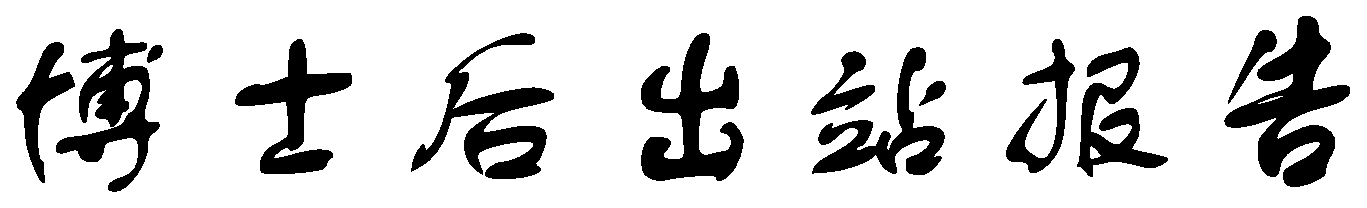
\includegraphics[width=12.8cm]{postdoc1.eps}
\end{center}

\vspace{0.15cm}

\begin{center}
{\erhao\song{\bf 联邦学习中模型个性化算法研究}}
\end{center}

\vspace{0.05cm}

\begin{spacing}{2}
\begin{center}{\erhao\bf
Study of Model Personalization Methods in Federated Learning}
\end{center}
\end{spacing}

\vspace{0.05cm}

\begin{center}
{\xiaoerhao\song\boldmath\bf 文豪}
\end{center}

\vspace{0.15cm}

\begin{tabbing} %tabbing 列表

\hspace*{3cm} \= \hspace{2.6cm} \= \kill
% \= in tabbing environment, sets a tab stop
% \kill in a\tabbing environment, deletes previous line so tabs can be set without outputting text.
% \> in tabbing environment is a forward tab.
% 这次的居中 用的 \centering ,注意三次的区别。
\>{\song\sihao\textbf {研\hspace{0.3cm}究\hspace{0.3cm}方\hspace{0.3cm}向\hspace{0.3cm} :}} \>
{\centering\song\sihao\textbf{~~~~~~~~~~联邦学习~~~~~~~~~~~~~}}\\
% 总长3.4cm
\\
\>{\song\sihao\textbf {合\hspace{0.3cm}作\hspace{0.3cm}导\hspace{0.3cm}师\hspace{0.3cm} :}}\>
{\centering\song\sihao\textbf{~~~~~~~~~~韩德仁~~~~教授~~~~~~~~~~~}} \\
\\
\>{\song\sihao\textbf {工作完成日期 \ \ :}}\> {\centering\song\sihao\textbf{~~~~~~~~~~2021年3月 --- 2023年6月~~~~~~~~~~}}\\
\\
\>{\song\sihao\textbf {报告提交日期 \ \ :}}\> {\centering\song\sihao\textbf{~~~~~~~~~~2023 年6月~~~~~~~~~~}} \\

\end{tabbing}

\vspace{0.1cm}
\begin{center}
{\song\boldmath \sihao ~2023~年~6~ 月}
\end{center}


\newpage
~~~\vspace{1em}
\thispagestyle{empty}

\pagenumbering{Roman}

% \newcommand{\upcite}[1]{\textsuperscript{\textsuperscript{\cite{#1}}}}

\baselineskip 18.8pt

% clear the extra empty page caused by the above \newpage command
\makeatletter\@openrightfalse

\chapter*{摘~~~要}
\headheight=15.24pt%5mm
\markboth{摘~~~要}{摘~~~要}
\addcontentsline{toc}{chapter}{{{\hei 摘~要}}\numberline ~}
\addcontentsline{toe}{chapter}{{{Abstract in Chinese}}\numberline ~}

\pagenumbering{Roman}\setcounter{page}{1}

% finished

联邦学习是伴随着去中心化、保护隐私等需求而兴起的一种人工智能的技术。它是一种全新的机器学习范式,适用于有中心节点居中协调,多个子节点进行协作参与,进行联合建模的场景。在这种场景下,联邦学习的方法能够在每个参与方不暴露己方拥有的数据的情况下,完成协同建模的任务。目前,联邦学习已成为了机器学习、人工智能领域的一个活跃的分支领域。

本文主要关注的是联邦学习中的优化算法及其在个性化联邦学习当中的应用。本文首先详细介绍联邦学习相关的多种优化算法,特别是分解算法。分解算法基本思想是将大规模的问题分解成一系列小规模的问题,将每个子问题分开处理,使得迭代算法中的子问题更容易求解或者更容易并行化。典型的分解算法包括了算子分裂法、交替方向乘子法等。目前已经有了一系列的工作,展现了分解算法在联邦学习问题研究中的独特优势。

随后,本文介绍个性化联邦学习特有的一些算法,并将分解算法应用于个性化联邦学习问题的研究。个性化联邦学习是处理具有复杂数据分布的联邦学习问题的一种方法,在协同训练公共模型的同时,允许参与方得到保留个性化特征、稍有差异的本地模型,提升了相关复杂场景下联邦学习的适用性。个性化联邦学习在问题建模、算法设计等方面仍有大量未解决的问题,本文将在这些问题上进行深入探讨,形成一些独到的研究。

最后,文本将介绍为联邦学习算法效果验证设计的一套仿真系统,并用此仿真系统进行数值实验,并与已有的一些算法形成对比,验证本文提出算法的效果。

\par
\bigskip

{\song \textbf{关键词}: 联邦学习, 协同建模, 分解算法, 算子分裂法, 模型个性化}

% \newpage
% ~~~\vspace{1em}
% \thispagestyle{empty}


\makeatletter\@openrighttrue

\chapter*{{Abstract}}%\vskip1cm
 \headheight=15.24pt%5mm
\markboth{Abstract} {Abstract}
 \headheight=15.24pt%5mm
\addcontentsline{toc}{chapter}{{{\bf Abstract}}\numberline ~~~}
\addcontentsline{toe}{chapter}{{{\bf Abstract in English}}\numberline ~}
\pagenumbering{Roman}\setcounter{page}{2}

% finished

Federated learning is an artificial intelligence technology that has emerged with the need for decentralization and privacy protection. It is a brand-new machine learning paradigm for scenarios where a central node (the server) coordinates multiple sub-nodes (the clients) into a collaborative modelling task. In this scenario, the participants can accomplish the task of collaborative modelling without exposing their private data. Currently, federated learning has become an active branch of machine learning and artificial intelligence.

This thesis mainly focuses on optimization algorithms in federated learning and their application in personalized federated learning. This thesis first introduces existing optimization algorithms in federated learning in detail, especially the decomposition algorithms. The basic idea of the decomposition algorithm is to decompose a large-scale problem into a series of small-scale problems and process each sub-problem separately so that the sub-problems in the iterative algorithms are easier to solve or easier to parallelize. Typical decomposition algorithms include operator splitting methods, alternating direction multiplier methods, etc. There are already a series of works showing the unique advantages of decomposition algorithms in the study of federated learning problems.

Subsequently, this thesis introduces algorithms for personalized federated learning and applies the decomposition algorithms to the research of personalized federated learning problems. Personalized federated learning is a method to deal with federated learning problems with complex data distribution. While training a public model collaboratively, it allows participants to obtain slightly different local models that retain their local characteristics, which improves the applicability of federated learning in related complex scenarios. There are still a lot of open problems in modelling and algorithm design in personalized federated learning. This thesis will conduct in-depth discussions on these problems and propose new algorithms and perspectives.

This thesis finishes with the introduction of a new simulation system designed for the verification of the federated learning algorithms, and numerical experiments using this simulation system to validate the algorithms proposed in this thesis in comparison to some existing algorithms.

\par
\bigskip

{\bf Key words:} Federated Learning, Collaborative Modeling, Decomposition Algorithms, Operator Splitting Methods, Model Personalization

%\nopagebreak[4]
\newpage
~~~\vspace{1em}
\thispagestyle{empty}



%\mbox{}\newpage
\chapter*{符~号~说~明}
\headheight=15.24pt%5mm
\addcontentsline{toc}{chapter}{\numberline {{\heiti 符~号~说~明}}~~~}
\addcontentsline{toe}{chapter}{{{\bf Notation}}\numberline~}
\markboth{符~号~说~明}{北京航空航天大学文豪博士后研究工作报告}
%%%%%%%%%%%%%%%%%%%%%%%%%%%%%%%%%%%%%%%%%%%%%%%%%%%%%%%%%5
这里给出本文常用的一些符号, 未包含其中的符号将在文中用到时具体说明.
\begin{equation*}
  \begin{array}{lll}
\mathbb{R}&\qquad\qquad\qquad\qquad\qquad&\text{实数集}\\
\mathbb{C}&&\text{复数集}\\
\mathbb{R}^{n} &&\text{实~$n$ 维列向量集} \\
\mathbb{C}^{n} &&\text{复~$n$ 维列向量集} \\
\mathbb{R}^{m\times n} && \text{实~$m\times n$ 矩阵的集合} \\
\mathbb{C}^{m\times n} && \text{复~$m\times n$ 矩阵的集合} \\
%\mathbf{0}&& \text{零向量或零矩阵}\\
%\nabla &&\text{梯度算子} \\
%\nabla \cdot  &&\text{散度算子} \\
%%\nabla \times  &&\text{旋度算子} \\
%\Delta  &&\text{拉普拉斯算子} \\
\mathrm{i}&&\text{虚单位}\\
\overline{\theta} && \text{复数~$\theta$~的共轭}\\
|\cdot| &&\text{实数的绝对值或复数的模}\\
I_n~\text{或}~I &&\text{($n$~阶)单位矩阵}\\
O_n~\text{或}~O &&\text{($n$~阶)零矩阵}\\
A^\mathrm{T} &&\text{矩阵~$A$~的转置矩阵}\\
A^* &&\text{矩阵~$A$~的共轭转置矩阵}\\
A^{-1}&&  \text{矩阵~$A$~的逆矩阵}\\
\sigma(A)&&\text{矩阵~$A$~的谱集}\\
\rho(A) &&\text{矩阵~$A$~的谱半径}\\
\nu(A) &&\text{矩阵~$A$~的拟谱半径}\\
%\lambda_{\min}(A)&&\text{矩阵~$A$~的最小特征值}\\
%\lambda_{\min}^+(A)&&\text{矩阵~$A$~的最小正特征值}\\
%\lambda_{\max}(A)&&\text{矩阵~$A$~的最大特征值}\\
\mathrm{rank}(A)&&\text{矩阵~$A$~的秩}\\
\mathrm{null}(A)&&\text{矩阵~$A$~的零空间}\\
\mathrm{range}(A)&&\text{矩阵~$A$~的值域}\\
\mathrm{index}(A)&&\text{矩阵~$A$~的指标}\\
%\mathrm{tr}(A)&&\text{矩阵~$A$~的迹}\\
A\otimes B&&\text{矩阵~$A$~和~$B$~的\,Kronecker\,积}\\
\|\cdot\|_2&&\text{向量或矩阵的~$2$-范数}\\
%\|\cdot\|_A$$ && \text{向量的~$A$-范数}\\
%\|\cdot\|_F&&\text{矩阵的\,Frobenius\,范数}\\
A\succ O&&\text{矩阵\,$A$\,为对称正定矩阵}\\
\mathrm{span}\{x_1,\cdots,x_n\}&&\text{向量~$x_1,\cdots,x_n$~张成的线性空间}
\end{array}
\end{equation*}
\nopagebreak[4]


\setcounter{tocdepth}{1}  % no subsections?
\tableofcontents
\tableofengcontents
\mainmatter

%\mbox{}\newpage
\chapter{\hspace{-1mm}\bf 绪论及预备知识}
\label{chap1}
\addcontentsline{toe}{chapter}{{{\bf Chapter \thecurrentchapter \ 
Introduction and Preliminaries }}\numberline\,}
\markboth{第 \thecurrentchapter 章\ \ 
绪论及预备知识}{北京航空航天大学博士后研究工作报告}

%%%%%%%%%%%%%%%%%%%%%%%%%%%%%%%%%%%%%%%%%%%%%%%%%%%%%%%%%%%


\section{绪论}
\addcontentsline{toe}{section}{{1.1\ \ Introduction}\numberline\,}
\label{sec:chap1-introduction}

% finished

随着人工智能(Artificial Intelligence, AI)、大数据(Big Data)等技术的飞速发展,特别是物联网(Internet of Things, IoT)的快速普及,可用于机器学习研究的数据呈爆发式增长,其来源与分布的形式,以及来自实际应用的需求也越来越多样化。这种变化趋势给机器学习的研究与应用带来了前所未有的挑战,也提供了崭新的发展机遇。

传统上来说,机器学习的范式是将要研究的数据集中到一起,例如一个数据中心,进行统计分析、建模方法、优化算法等方面的研究。然而随着上文提到的研究数据来源与分布的形式的多样化,以及法律法规等其他因素的制约,将数据集中到一起面临越来越大的困难。举例来说,执行某一类任务的物联网设备往往数量庞大,数量级以百万乃至千万计,其产生的数据总量巨大。但是物联网设备的通信带宽往往不高,相互之间的通信,以及与数据中心之间的通信往往会有较高的延迟。在这种场景下,将感兴趣的数据集中到一起进行研究,是极其困难,成本非常高的。与此同时,随着人们的隐私保护意识越来越强,相关的法律法规,例如欧盟2018年正式生效的《General Data Protection Regulation》,越来越严格,收集用户的数据也越来越困难\citep{Albrecht_2016}。例如,用户的键盘输入数据可以用于训练输入自动补全的模型,提高用户输入效率\citep{fl_keyboard}。一般来说,通信带宽不是这类数据共享的瓶颈,但是基于隐私法律法规的限制,收集此类数据限制极大。还有一些类型的数据是具有高度机密性的数据,例如医疗、金融数据。相关的医疗机构之间或者金融机构之间往往不会进行数据共享。

在很多场景下,数据孤岛的效应比较突出:各个数据持有方持有的数据量严重不平衡,分布差异性大。如果各个数据持有方仅仅依赖各自拥有的本地数据进行模型训练,得到的机器学习模型往往是严重过拟合的,实际使用效果往往不佳。

因此,如何在尽可能地保证质量以及不进行敏感数据传输的前提下,高效率地进行分布式的机器学习模型的训练,同时使得每一个参与方都获得模型效果提升等形式的收益,最大限度的利用大数据带来的便利与优势,这一问题的重要性越来越突出。因为场景的多样性,或者说数据分布的多样性,以及相应需求的多样性,一个普适的、能满足所有需求的分布式机器学习模型训练的范式是不存在的,很多时候必须有侧重地针对某一部分需求设计相应的分布式学习方法,例如侧重隐私性的差分隐私方法(Differential Privacy)\citep{Dwork_2008_DP}, 侧重模型训练效果的优化算法设计\citep{boyd2011distributed}等。这些问题还有很多亟待改进与完善,具有关阔的研究前景与巨大的应用价值。


\section{联邦学习的起源与演化}
\addcontentsline{toe}{section}{{\thecurrentchapter .2\ \ Origin and Development of Federal Learning}\numberline\,}
\label{sec:chap1-fl-origin}

% almost finished
% indexed

联邦学习Federated Learning\index{联邦学习, Federated Learning}这个名词首次由Google的研究人员McMahan等人于2016年在文章\emph{Communication-Efficient Learning of Deep Networks from Decentralized Data}\cite{mcmahan2017fed_avg}中提出:
\begin{quote}
    ``We term our approach Federated Learning, since the learning task is solved by a loose federation of participating devices (which we refer to as clients) which are coordinated by a central server.''
\end{quote}
文章\parencite{mcmahan2017fed_avg}最初目的,是希望能利用用户手机端的数据改进安卓手机上输入法的预测,在防止数据泄露的前提下,基于分布在多个设备上的数据集构建机器学习模型\cite{hard2018_fl_keyboard,yang2018_fl_google}。具有里程碑意义的综述文章\emph{Advances and Open Problems in Federated Learning}\cite{kairouz2019advances_fl} 给联邦学习下过如下的定义
\begin{quote}
    ``Federated learning is a machine learning setting where multiple entities (clients) collaborate in solving a machine learning problem, under the coordination of a central server or service provider. Each client's raw data is stored locally and not exchanged or transferred; instead, focused updates intended for immediate aggregation are used to achieve the learning objective.''
\end{quote}
也就是说,联邦学习是一种新的机器学习范式,适用于有中心节点 (Server) \index{中心节点, Server}居中协调,多个子节点 (Client) \index{子节点, Client}进行协作参与,进行联合建模的场景。在这种场景下,联邦学习的方法能够在每个参与方不暴露己方拥有的数据的情况下,完成联合建模的任务。一般来说,在联邦学习的框架下,数据拥有方在不用给出己方数据的情况下,也可进行模型训练得到公共的模型$M_{\text{fed}}$,使得模型$M_{text{fed}}$,与将数据集中到一起进行训练能得到的模型$M$,二者的预测值的偏差的期望能足够小。
\begin{equation}
\label{eq:general-fl}
\expectation_{z\sim\mathcal{D}} \lVert M_{text{fed}}(z) - M(z) \rVert \leqslant \delta.
\end{equation}
其中$\mathcal{D}$是总体训练数据的分布,$\delta$是某个我们能够接受的偏差的上界。尽管分布式优化 (Distributed Optimization) \index{分布式优化, Distributed Optimization}、加密计算等问题在联邦学习这一概念被提出之前就有学者进行了研究\cite{boyd2011distributed, dist_pca_2014_nips, Gentry_2009_FHE, Nikolaenko_2013}, 但是直到联邦学习被正式提出\cite{mcmahan2017fed_avg},以上关于联邦学习独有的一些特性以及需求才真正被学界以及工业界所重视,相关的研究才开始蓬勃发展。需要注意的是,尽管文献\parencite{kairouz2019advances_fl}给出的联邦学习的定义强调了有中心节点这一特征,同时大部分关于联邦学习的文献也是基于这一假设开展研究的,但仍有一部分关于联邦学习的文献是基于无中心的完全分布式的节点网络进行研究的\cite{elgabli2020gadmm, issaid2020cq-ggadmm}.

从上面关于联邦学习的定义中我们可以看出,一般来说,联邦学习的参与方构成了一个有中心的网络。我们在这里先明确关于这个网络的一些基本的术语:
\begin{itemize}
    \item Server: 中心节点,负责整个联邦学习网络的控制、编排子节点任务的工作,同时维护全局共享的模型,其本身一般没有训练数据;
    \item Client: 子节点,拥有一定数量的训练数据,利用这些数据以及中心节点共享的信息,执行本地模型训练的任务。
\end{itemize}

我国杨强教授领导的香港科技大学以及微众银行 (WeBank) 的AI研究团队,从经济金融行业实践出发,将文献\parencite{mcmahan2017fed_avg}考虑的联邦学习经典的应用场景,即超大规模的移动、边缘设备协同参与模型训练的场景,扩展到了多个数据不互通的数据中心的场景\cite{Yang_2019_VFL}。前者被抽象为了\textbf{跨设备} (Cross-Device) \index{跨设备, Cross-Device}的场景,后者被抽象为了\textbf{跨(数据)仓库} (Cross-Silo) \index{跨(数据)仓库, Cross-Silo}的场景\cite{kairouz2019advances_fl}。跨设备的场景具有子节点数量多,每个子节点持有数据量少,算力低,通信带宽低且不稳定,对通信开销非常敏感等特点;跨仓库的场景具有子节点数量少 (数量级通常在$10^2$以内),每个子节点持有数据量大,算力高,对数据的安全性、保密性要求高等特点,子节点与中心节点的通信开销与子节点本身的算力都可能成为瓶颈。这两种经过高度抽象的场景基本涵盖了联邦学习面临的所有的场景。文献\parencite{kairouz2019advances_fl}的Table 1对于这两种场景的联邦学习的特点进行了全面的总结与对比。

文献\parencite{Yang_2019_VFL}的另一个突出的贡献是从数据分布的角度,具体来说,是样本特征空间 (Sample Feature Space) \index{样本特征空间, Sample Feature Space}以及样本编号空间 (Sample ID Space) \index{样本编号空间, Sample ID Space}的角度,将联邦学习分为三类:横向联邦学习 (Horizontal Federated Learning, HFL) \index{横向联邦学习, Horizontal Federated Learning, HFL}、纵向联邦学习 (Vertical Federated Learning, VFL) \index{纵向联邦学习, Vertical Federated Learning, VFL}和联邦迁移学习 (Federated Transfer Learning, FTL) \index{联邦迁移学习, Federated Transfer Learning, FTL}。

横向联邦学习是最常见的一类联邦学习,即每个参与方数据的特征空间基本是一致的,但各自拥有的样本编号基本是不重叠的。一般情况下,我们谈论的联邦学习,以及跨设备的联邦学习,都是横向联邦学习。纵向联邦学习则正好与横向联邦学习相反,纵向联邦学习的每个参与方有重叠度较高的样本编号空间,但是参与方之间拥有的每个样本的特征的重叠度很低。这在金融风控等领域是非常常见的。联邦迁移学习则是迁移学习 (Transfer Learning) \index{迁移学习, Transfer Learning}这一概念在联邦学习这一范畴内的具体应用,首先于文献\parencite{liu_2020_transfer_fl}中被系统地研究。联邦迁移学习的核心思想是,源领域 (Source Domain) 和目标领域 (Target Domain) 之间的相似性,将机器学习模型从源领域学习到的知识迁移应用到目标领域。源领域往往是知识丰富的领域 (具有丰富的标签),而目标领域则是知识欠丰富,需要接受知识迁移的领域。联邦迁移学习天然适合于智慧医疗领域,例如不同医疗机构的医学影像数据一般都是不同的,但基础都是影像特征的提取与利用。

一般来说,假设一个联邦学习系统有$K$个参与方,每个参与方拥有的数据分布记作$\mathcal{D}_k,$ $k = 1, \ldots, K.$ $\mathcal{D}_k$有分解
\begin{equation*}
\mathcal{D}_k \subseteq \mathcal{X}_k \times \mathcal{Y}_k \times \mathcal{I}_k,
\end{equation*}
其中$\mathcal{X}_k$为数据样本的特征空间,$\mathcal{Y}_k$为数据样本的标签空间 (Sample Label Space) \index{样本标签空间, Sample Label Space},$\mathcal{I}_k$为数据样本编号空间。那么有\cite{Yang_2019_VFL,vfl}
\begin{itemize}
\item 横向联邦学习:
\begin{equation*}
\mathcal{X}_i \eqabove{d} \mathcal{X}_j, ~ \mathcal{Y}_i \eqabove{d} \mathcal{Y}_j, ~ \mathcal{I}_i \neqabove{d} \mathcal{I}_j, ~ \forall i \neq j;
\end{equation*}
以上的符号$\eqabove{d}$表示相应的概率空间是同分布的。横向联邦学习一般可以简化建模为如下的最优化问题\cite{kairouz2019advances_fl}
\begin{equation}
\label{eq:general-hfl}
\begin{array}{cl}
\text{minimize} & f(\theta) = \expectation\limits_{k \sim {\mathcal{P}}} [f_k(\theta)] = \sum\limits_{k=1}^K w_k f_k(\theta), \\
\text{where} & f_k(\theta) = \expectation\limits_{(x, y) \sim \mathcal{D}_k} [\ell_k(\theta; x, y)],
\end{array}
\end{equation}
其中符号$\expectation$表示关于分布的期望,$\theta$是模型参数,也就是我们的学习目标;$\mathcal{P}$是参与训练的节点的分布,这里我们假设了总共有$K$个节点;$w_k$是节点$k$的权重,一般与节点持有的数据量正相关;$\ell_k$是节点$k$上模型训练的损失函数 (Loss Function) \index{损失函数, Loss Function}或者目标函数 (Objective Function) \index{目标函数, Objective Function};$x, y$分别表示数据的特征与数据的标签。$f_k$以及$f$则被称作局部目标函数以及全局目标函数。这里,我们忽略了数据样本编号空间,将数据分布简写为了$(x, y) \sim \mathcal{D}_k \subseteq \mathcal{X}_k \times \mathcal{Y}_k.$
\item 纵向联邦学习:
\begin{equation*}
\mathcal{X}_i \neqabove{d} \mathcal{X}_j, ~ \mathcal{Y}_i \neqabove{d} \mathcal{Y}_j, ~ \mathcal{I}_i \eqabove{d} \mathcal{I}_j, ~ \forall i \neq j;
\end{equation*}
纵向联邦学习对应的最优化模型可以写为\cite{vfl}
\begin{equation}
\label{eq:general-vfl}
\begin{array}{cl}
\text{minimize} & f(\theta) = \sum\limits_{i=1}^N \mathcal{L} \left( \mathcal{F}_K \left( \psi_K; f_{1}(\theta_{1}; x_{i}^{(1)}), \ldots, f_{K}(\theta_{K}; x_{i}^{(K)}), y_{i} \right) \right), \\
\text{where} & \theta = (\theta_{1}, \ldots, \theta_{K}), ~ x_{i} = (x_{i}^{(1)}, \ldots, x_{i}^{(K)}),
\end{array}
\end{equation}
其中$N$是总样本数,也就是说我们有$N$条数据;$x_{i}^{(k)}$为参与联邦学习的节点$k$掌握的样本$i$的部分特征,所有节点掌握的样本$i$的特征按一定规则排列构成了样本$i$的总体特征$x_{i} = (x_{i}^{(1)}, \ldots, x_{i}^{(K)}).$ 样本$i$的标签一般都假设在某一个(例如节点$K$)参与纵向联邦学习训练的节点上,这个节点被称作积极节点 (Active Party),其余节点被称作被动节点 (Passive Parties)。 除了标签$y,$ 积极节点$K$上还拥有的直接与训练任务相关的所谓的全局模块 (Global Module) $\mathcal{F}_K,$ 其参数为$\psi_K.$ 全局模块可能是简单的求平均的模块,也可以是一个神经网络的最顶层的用于最终进行回归或者分类任务的全连接层。$\mathcal{L}$是训练任务的损失函数。
\item 联邦迁移学习:
\begin{equation*}
\mathcal{X}_i \neqabove{d} \mathcal{X}_j, ~ \mathcal{Y}_i \neqabove{d} \mathcal{Y}_j, ~ \mathcal{I}_i \neqabove{d} \mathcal{I}_j, ~ \forall i \neq j;
\end{equation*}
一个有$A, B$两方参与的联邦迁移学习可以简化为如下的模型\cite{liu_2020_transfer_fl}
\begin{equation}
\label{eq:general-ftl}
\text{minimize} \quad \sum_{i=1}^{N_{AB}} \left( \ell_1(y_i^A, \varphi(u_i^B)) + \lambda \ell_2(u_i^A, u_i^B)  \right),
\end{equation}
其中$A$是源领域,$B$是目标领域;$N_{AB}$是$A, B$两方共有的样本数量;$u_i^A, u_i^B \in \mathcal{U},$ $\mathcal{U}$是$A, B$两方共有的隐式特征表示空间(Hidden Representation Space),$A, B$两方的特征通过如下的映射(例如通过两个神经网络)映到同一个空间$\mathcal{U}$
\begin{gather*}
\mathcal{X}^A \to \mathcal{U}: ~ x_i^A \mapsto u_i^A, \\ \mathcal{X}^B \to \mathcal{U}: ~ x_i^B \mapsto u_i^B.
\end{gather*}
$\ell_1$是训练任务的损失函数,$\ell_2$是所谓的对齐损失函数 (Alignment Loss Function),可以取
\begin{equation*}
- \langle u_i^A, u_i^B \rangle, ~~ \text{或者} ~ \lVert u_i^A, u_i^B \rVert^2.
\end{equation*}
$\varphi$是一个所谓的翻译函数 (Translator Function),用于对$u_i^B$进行打标签的,一般也可以利用隐式表示特征的相关性取作
\begin{equation}
\label{eq:ftl-translator-func}
\varphi(u_i^B) = \frac{1}{N_A} \sum\limits_{i=1}^{N_A} y_i^A \langle u_i^A, u_i^B \rangle,
\end{equation}
其中$N_{A}$是源领域$A$拥有的样本数量。
\end{itemize}
我们可以用图\ref{fig:three-types-fl}~来概括地表示这三类联邦学习在以上几种概率空间上的特点。

\begin{figure}[H]
\centering
\begin{boxedminipage}{0.95\textwidth}
\centering
\begin{minipage}{0.29\textwidth}
\begin{tikzpicture}
\draw (0, 0) rectangle (3.8, 4.5);
\node at (1.95, 5.5) {横向联邦学习};
\draw[fill=pink] (0, 0) rectangle (3.5, 1.1) node[pos=.5] {client $i$};
\draw[fill=green] (0.2, 3.3) rectangle (3.8, 4.5) node[pos=.5] {client $j$};
\draw[fill=yellow] (0.3, 0.9) rectangle (3.7, 3.6) node[pos=.4] {client $k$};
\node at (1.95, -0.4) {样本特征空间};
\end{tikzpicture}
\end{minipage}
\begin{minipage}{0.29\textwidth}
\begin{tikzpicture}
\draw (0,0) rectangle (3.8, 4.5);
\node at (1.95, 5.5) {纵向联邦学习};
\draw[fill=pink] (0, 0) rectangle (1.4, 4.2) node[pos=.5, rotate=-90] {client $i$};
\draw[fill=green] (1.95, 0) rectangle (3.8, 4.5) node[pos=.5, rotate=-90] {client $j$};
\draw[fill=yellow] (1.3, 0.2) rectangle (2.1, 4.4) node[pos=.4, rotate=-90] {client $k$};
\node at (1.95, -0.4) {样本特征空间};
\end{tikzpicture}
\end{minipage}
\begin{minipage}{0.29\textwidth}
\begin{tikzpicture}
\draw (0,0) rectangle (3.8, 4.5);
\node at (1.95, 5.5) {联邦迁移学习};
\draw[fill=yellow] (0.9, 1.2) rectangle (2.2, 4.1) node[pos=.5] {client $k$};
\draw[fill=pink] (0, 0) rectangle (1.3, 1.6) node[pos=.5] {client $i$};
\draw[fill=green] (1.9, 3.6) rectangle (3.8, 4.5) node[pos=.5] {client $j$};
\node at (1.95, -0.4) {样本特征空间};
\end{tikzpicture}
\end{minipage}
\begin{minipage}{0.05\textwidth}
\begin{tikzpicture}
% \coordinate (sample_node) at (0,0);
% \node[text width=1, left=0.5cm of sample_node.west] at () {样本维度};
\node[rotate=-90] () {样本编号空间};
\end{tikzpicture}
\end{minipage}
\end{boxedminipage}
\caption{三类联邦学习的样本特征空间与样本编号空间分布的示意图}
\label{fig:three-types-fl}
\end{figure}


一般来说,一个完整的联邦学习的迭代流程可以归纳如下
\begin{itemize}
    \item 子节点选取 (Client Selection);
    \item 中心节点将子节点计算需要的信息(例如模型参数、梯度等)下发到被选取的子节点 (Parameter Broadcast);
    \item {\bfseries 子节点执行本地计算,更新本地模型参数 (Local Parameter Update);}
    \item 子节点将更新后的信息返回中心节点,中心节点将收集到的信息进行聚合 (Parameter Aggregation);
    \item {\bfseries 中心节点执行计算,更新全局模型 (Global Parameter Update)。}
\end{itemize}
可以看到,这一流程关于模型参数的更新完全是解耦合的,因此子节点模型更新方法与中心节点的全局模型的更新方法可以做相对灵活的组合,只要中心节点与子节点之间定义好了传输信息的协议。我们可以把以上的流程用图\ref{fig:broadcast-local-update}~与图\ref{fig:agg-global-update}~来进行简单的示意。

\tikzset{%
  client/.style={
    rectangle,
    thick,
    draw,
    minimum size=0.7cm,
    text width=1cm,
    align=center
  },
  client missing/.style={
    draw=none,
    scale=2,
    text height=0.333cm,
    execute at begin node=$\cdots$
  },
}

\begin{figure}[ht]
\centering
% \begin{tikzpicture}[scale=2.1]
\begin{scaletikzpicturetowidth}{0.95\textwidth}
\begin{tikzpicture}[scale=\tikzscale]
\node[client] at (0, 0) (server) {server $\theta$};
\node[client, below left = 1.5cm and 3.5cm of server.south] (client-1) {client $\theta_1$};
\node[client, right = 0.4cm of client-1.east] (client-2) {client $\theta_2$};
\node[client, right = 0.4cm of client-2.east] (client-3) {client $\theta_3$};
\node[client missing, right = 0.1cm of client-3.east] (client-missing) {};
\node[client, right = 0.1cm of client-missing.east] (client-n) {client $\theta_K$};
\path[-{Stealth}] ([xshift=-0.5cm,yshift=-0.1cm]server.south) edge ([yshift=0.15cm]client-1.north);
\path[-{Stealth}] ([xshift=-0.2cm,yshift=-0.1cm]server.south) edge ([yshift=0.15cm]client-2.north);
\path[-{Stealth}] ([xshift=0.05cm,yshift=-0.1cm]server.south) edge ([yshift=0.15cm]client-3.north);
\path[-{Stealth}] ([xshift=0.4cm,yshift=-0.1cm]server.south) edge ([yshift=0.15cm]client-n.north);
\node[text width=1.2cm, align=center, right=0.3cm of client-n.east] (local-update) {local update};
\node[text width=1.8cm, align=center, above left=0.5cm and 0.1cm of local-update.north] () {params broadcast};
\end{tikzpicture}
\end{scaletikzpicturetowidth}
\caption{中心节点将信息下发到子节点,子节点执行本地模型参数更新}
\label{fig:broadcast-local-update}
\end{figure}

\begin{figure}[ht]
\centering
% \begin{tikzpicture}[scale=2.1]
\begin{scaletikzpicturetowidth}{0.95\textwidth}
\begin{tikzpicture}[scale=\tikzscale]
\node[client] at (0, 0) (server) {server $\theta$};
\node[client, below left = 1.5cm and 3.5cm of server.south] (client-1) {client $\theta_1$};
\node[client, right = 0.4cm of client-1.east] (client-2) {client $\theta_2$};
\node[client, right = 0.4cm of client-2.east] (client-3) {client $\theta_3$};
\node[client missing, right = 0.1cm of client-3.east] (client-missing) {};
\node[client, right = 0.1cm of client-missing.east] (client-n) {client $\theta_K$};
\path[-{Stealth}] ([yshift=0.15cm]client-1.north) edge ([xshift=-0.5cm,yshift=-0.1cm]server.south);
\path[-{Stealth}] ([yshift=0.15cm]client-2.north) edge ([xshift=-0.2cm,yshift=-0.1cm]server.south);
\path[-{Stealth}] ([yshift=0.15cm]client-3.north) edge ([xshift=0.05cm,yshift=-0.1cm]server.south);
\path[-{Stealth}] ([yshift=0.15cm]client-n.north) edge ([xshift=0.4cm,yshift=-0.1cm]server.south);
\node[text width=1.2cm, align=center, right=0.3cm of server.east] (global-update) {global update};
\node[text width=1.8cm, align=center, below right=0.25cm and 0.1cm of global-update.south] () {aggregation};
\end{tikzpicture}
\end{scaletikzpicturetowidth}
\caption{中心节点收集子节点更新的信息,并执行全局模型参数更新}
\label{fig:agg-global-update}
\end{figure}



\section{联邦学习的应用与发展前景}
\addcontentsline{toe}{section}{{1.3\ \ Applications and Future Perspective of Federal Learning}\numberline\,}
\label{sec:chap1-fl-applications}

尽管联邦学习这一概念被提出\cite{mcmahan2017fed_avg}的时间不长,但是联邦学习已经有了不少实际的应用。我们这里仅列举一些比较重要的例子。
\begin{itemize}
    \item 首先是金融领域,联邦学习在财会\cite{Schreyer_2022_fl_audits},信贷风控\cite{Imteaj_2022_fl},反欺诈\cite{Lv_2021_fl},防范金融犯罪\cite{Toyotaro_2019_fl}等各个方面都有了实际的应用。这其中最引人注目的当属我国微众银行在这一领域的一系列前沿以及开创性的研究\cite{Yang_2019_VFL, liu_2020_transfer_fl, vfl},并以真正落地形成工业级产品的联邦学习应用框架FATE\cite{liu_2021_fate_fl}.
    \item 联邦学习在智慧医疗领域也有颇多成功应用的案例\cite{rauniyar2022_fl_medical, Antunes_2022_fl_healthcare}。从电子健康档案(Electronic Health Records, EHR)处理\cite{Brisimi_2018_fl_ehr},医学影像处理\cite{Li_2020_fl_mri},到新冠(COVID-19)等流行病的研究\cite{Dayan_2021_fl_covid},都有联邦学习的应用案例。医学因为其数据隐私性的严格要求,同时又有市场的巨大需求驱动,是联邦学习非常适宜的应用领域,同时也可能是相关研究最活跃、应用落地最多的领域之一。
    \item 移动设备、物联网领域:这是联邦学习发轫\cite{mcmahan2017fed_avg}的领域,也是大规模跨设备(Cross-Device)场景最常见的领域,应用也从最一开始的安卓设备键盘辅助输入扩展到了移动设备的语音处理\cite{Leroy_2019_fl_ks},人体活动识别(Human Activity Recognition)\cite{Sozinov_2018_fl_human},乃至人口流动预测(Human Mobility Prediction)\cite{feng_2020_fl_pmf}等问题。因为隐私性以及模型个性化(Model Personalization)等要求,很多时候联邦学习甚至是解决问题的唯一选择。
\end{itemize}

除了以上列举的一些领域外,联邦学习的应用还逐渐扩大到了智慧城市(Smart City)\cite{Zheng_2021_fl_smart_city}纳米材料\cite{Huang_2022_fl_physics}等全新的领域。可以说,联邦学习的应用场景相较于它被提出时已经得到了极大的丰富,用于仿真试验的数据集也有了很多积累。同时,也涌现出了像FedML\cite{he_2020_fedml},TensorFlow Federated\cite{tensorflow},FedSim\cite{wu_2021_fedsim},PySyft\cite{ryffel_2018_pysyft},以及之前提到的FATE\cite{liu_2021_fate_fl}等多个有不同侧重点的联邦学习软件包,为联邦学习的研究与应用落地,都提供了极大的便利。然而目前联邦学习在理论以及实际应用上,还有不少问题没有完善的解决,仍然面临着诸多的挑战\cite{kairouz2019advances_fl, Li_2020_fl_challenges}。综述性的文章\parencite{Li_2020_fl_challenges}

待写。。。。


\section{本文结构}
\addcontentsline{toe}{section}{{1.4\ \ Structure of the Thesis}\numberline\,}
\label{sec:chap1-structure}

待写。。。。


%\mbox{}\newpage
\chapter{\hspace{-1mm}\bf 联邦学习中的优化算法}
\label{chap2}
\addcontentsline{toe}{chapter}{{{\bf Chapter 2\ \
Optimization Algorithms in Federated Learning }}\numberline\,}
\markboth{第\,2\,章\ \
待写}{北京航空航天大学博士后研究工作报告}

%%%%%%%%%%%%%%%%%%%%%%%%%%%%%%%%%%%%%%%%%%%%%%%%%%%%%%%%%%%

\section{联邦学习中的优化算法}
\addcontentsline{toe}{section}{{2.1\ \ Overview of Optimization Algorithms in Federated Learning}\numberline\,}
\label{sec:chap2-overview}

优化算法自从联邦学习这一概念诞生起,便一直是相关研究的中心问题之一。联邦学习开创性的文献\parencite{mcmahan2017fed_avg}中,最重要也是最为人所熟知的便是优化算法\texttt{FederatedAveraging}(简记为\texttt{FedAvg})的提出。这种算法的核心思想,是充分利用子节点的计算能力,在执行完一定轮数的随机梯度下降(Stochastic Gradient Descent, SGD)之后,由中心节点收集各子节点发送过来的模型参数,进行平均(Averaging),之后再将平均之后的模型参数广播(Broadcast)给子节点进行下一轮迭代。这样,规避了每一轮SGD都进行通信带来的巨大的通信开销,在加速模型训练的同时,数值上在某些情况下还有更好的收敛性。这实际上是一种比较朴素与简单的``跳步''的思想,这种思想也在随后的研究\cite{zhang2020fedpd, proxskip, proxskip-vr}也得到了进一步的发展。

联邦学习优化算法最重要的设计原则,是计算效率以及通信效率并重,甚至很多时候通信效率是更重要的一个方面。这也是联邦学习与传统的分布式优化(Distributed Optimization)最显著的区别之一。实际上,分布式优化在联邦学习被提出之前就是一个被研究得比较多的问题,从具体的问题,例如分布式主成分分析(Principal Component Analysis, PCA)\cite{dist_pca_2014_nips},到一般的算法理论\cite{boyd2011distributed}都有研究人员进行了研究。当时这些研究往往仅从计算效率以及效果出发,往往不考虑通信效率、通信保密性等问题。文献\parencite{mcmahan2017fed_avg}正是从实际问题出发,发现了这些需求,基于一种分布式梯度下降算法\cite{chen2016_revisit}(该算法在文献\parencite{mcmahan2017fed_avg}中被称作\texttt{FedSGD}算法),做了上文提到的改进而提出了\texttt{FedAvg}算法。

这里还需要强调的是,\texttt{FedAvg}相对于\texttt{FedSGD}的另一个关键的改进是,子节点与中心节点之间传输的信息,从梯度改为了模型参数。这在某种程度上规避了从梯度泄露联邦学习参与方私密训练数据\cite{zhu2019deep_leakage}的潜在风险。

沿用式\eqref{eq:general-hfl}中的记号,本文考虑联邦学习中的优化问题,其最基本的格式如下
\begin{equation}
\label{eq:fl-basic-dist}
\begin{array}{cl}
\minimize\limits_{\theta \in \R^d} & f(\theta) = \expectation\limits_{k \sim {\mathcal{P}}} [f_k(\theta)], \\
\text{where} & f_k(\theta) = \expectation\limits_{(x, y) \sim \mathcal{D}_k} [\ell_k(\theta; x, y)],
\end{array}
\end{equation}
假设我们令$\mathcal{P} = \{1, 2, \ldots, K\},$ 则上述模型可以简记为
\begin{equation}
\label{eq:fl-basic}
\begin{array}{cl}
\minimize\limits_{\theta \in \R^d} & f(\theta) = \sum\limits_{k=1}^K w_k f_k(\theta).
\end{array}
\end{equation}
对于$f$以及$f_k,$ 我们一般都假设它满足如下几条最基本的性质
\begin{itemize}
\item[(A1)] $f$以及$f_k$都是$L-$光滑的($L-$smooth),即
\begin{equation}
\label{eq:l-smooth}
\begin{array}{c}
\lVert \nabla f (\theta) - f (\theta') \rVert \leqslant L \lVert \theta - \theta' \rVert, \\
\lVert \nabla f_k (\theta) - f_k (\theta') \rVert \leqslant L \lVert \theta - \theta' \rVert,
\end{array}
~ \forall \theta, \theta' \in \R^d, k = 1, \ldots, K.
\end{equation}
\item[(A2)] $f$下有界(Lower Bounded):存在常数$c \in \R,$ 使得
\begin{equation}
\label{eq:lower-bounded}
f(\theta) \geqslant c > -\infty, ~ \forall \theta \in \R^d.
\end{equation}
\end{itemize}
很多时候,为了方便收敛性的分析,我们还会对目标函数的梯度进行一些假设
\begin{itemize}
\item[(A3)] 梯度有界性(Bounded Gradient):存在常数$G > 0,$ 使得
\begin{equation}
\label{eq:bdd_grad}
\lVert \nabla f_k (\theta) \rVert^2 \leqslant G^2, ~ \forall \theta \in \R^d, ~ k = 1, \ldots K.
\end{equation}
\end{itemize}
数据分布的特征(是否独立同分布,以及非独立同分布的程度)是联邦学习避免不了要考虑的问题,这也是联邦学习区别于传统的分布式优化的重要特征,这也是我们在\S\ref{sec:chap1-fl-applications}~中着重讨论过的问题。
\begin{itemize}
\item[(A4-1)] 数据独立同分布(I.I.D.):
\begin{equation}
\label{eq:iid-1}
\expectation\limits_{(x, y) \sim \mathcal{D}_k}[\nabla \ell_k(\theta; x, y)] = \nabla f(\theta), ~ \forall \theta \in \R^d, ~ k = 1, \ldots K,
\end{equation}
% 或者
% \begin{equation}
% \label{eq:iid-2}
% \sum\limits_{k=1}^K \expectation\limits_{(x, y) \sim \mathcal{D}_k}[\nabla f_k(\theta; x, y)] = \nabla f(\theta), \forall \theta \in \R^d, ~ k = 1, \ldots K,
% \end{equation}
\item[(A4-2)] 数据非独立同分布(Non-I.I.D.),这个时候我们需要有一个量,用来度量这种统计上的异质性的程度。这个量可以有多种定义方式,本文采用文献\parencite{karimireddy2020scaffold}以及文献\cite{zhang2020fedpd}中定义的梯度差异有界性(Bounded Gradient Dissimilarity),记作$(G; B)$-BGD. 具体来说,存在常数$G > 0,$ 以及$B \geqslant 0,$ 满足
\begin{equation}
\label{eq:bdd_grad_dissim}
\dfrac{1}{K} \sum\limits_{k=1}^K \lVert \nabla f_k(\theta) \rVert^2 \leqslant G^2 + B^2 \lVert \nabla f(\theta) \rVert^2, ~ \forall \theta \in \R^d.
\end{equation}
需要注意的是,如果令$B = 0,$ 那么梯度差异有界性条件\eqref{eq:bdd_grad_dissim}就退化为了梯度有界性条件\eqref{eq:bdd_grad}。
\end{itemize}

更方便以及自然的做法,是将问题\eqref{eq:fl-basic}写成约束优化问题的格式:
\begin{equation}
\label{eq:fl-basic-constraint}
\begin{array}{cl}
\begin{array}{cl}
\minimize\limits_{\theta \in \R^d} & f(\theta) = \sum\limits_{k=1}^K w_k f_k(\theta_k), \\
\text{subject to} & \theta_k = \theta, ~ k = 1, \ldots, K.
\end{array}
\end{array}
\end{equation}
我们很容易看出\eqref{eq:fl-basic-constraint}与\eqref{eq:fl-basic}这两种格式的等价性。格式\eqref{eq:fl-basic-constraint}再分布式优化中被称作共识问题(Consensus Problem)。

% 这里还应当着重指出的是,待写。。。。


\section{联邦学习中的临近点算法}
\addcontentsline{toe}{section}{{2.2\ \ Proximal Point Algorithms in Federated Learning}\numberline\,}
\label{sec:chap2-ppa}

基于减小数据非独立同分布情形下,每一轮的子节点更新对整体模型的影响,文献\parencite{sahu2018fedprox}首先提在子节点上的局部模型中增加邻近项的\texttt{FedProx}算法,达到了算法收敛更快、更加稳定的目的。具体来说,在算法迭代的第$t+1$轮,每个子节点优化的目标函数从$f_k(\theta_k)$变为了如下的带临近项的函数
\begin{equation}
\label{eq:fedprox}
f_k(\theta_k) + \frac{\mu}{2} \lVert \theta_k - \theta^{(t)} \rVert^2
\end{equation}
值得注意的是,上式临近项的中心为$\theta^{(t)},$ 即上一轮迭代得到的全局模型。关于临近项中心的其他选取,文献\parencite{hanzely2020federated,li_2021_ditto}进行了研究,我们随后进行详细介绍。

待写。。。。


% fedprox
bounded dissimilarity:
for some $\epsilon > 0$, $\exists B_{\epsilon}$ s.t. $\forall w \in \{ w ~|~ \lVert \nabla f(w) > \epsilon \rVert \}$, $B(w) \leqslant B$.

一些关于FedProx文章中的Theorem 4的观察:

在$\lVert \nabla f \rVert$的零点附近,如果这个零点没有被$\mathbb{E}_k[\lVert \nabla F_k \rVert]$消除掉的话,$B$会急速趋向于无穷,导致在$\lVert \nabla f \rVert$的零点附近,$\rho > 0$的假设不再成立,那么定理中的不等式就变得无意义了。当子节点之间的数据分布完全一致的时候(理想情况下),$B$恒为1,就不会有这个问题。这也是FedSplit\cite{pathak2020fedsplit}文章里提到的。


\input{content/chapter2/sec3-primal-dual}

\section{联邦学习中的算子分裂算法}
\addcontentsline{toe}{section}{{2.3\ \ Operator Splitting Algorithms in Federated Learning}\numberline\,}
\label{sec:chap2-operator-split}

% almost finished
% indexed

我们已经讨论过的通用加速技巧\cite{reddi2020fed_opt},方差缩减技术\cite{karimireddy2020scaffold},以及临近点方法\cite{sahu2018fedprox},解决的都是联邦学习在各种各样场景下的收敛性、收敛率相关的问题,而算法收敛结果的正确性这一问题始终没有得到重视。我们来举一个非常简单的例子来说明这个问题。

\begin{example}
\label{eg:correctness}
假设我们要拟合线性模型$y = mx$, $m$为需要拟合的变量,使用均方误差 (Mean Squared Error, MSE)\index{均方误差, Mean Squared Error, MSE} 做损失函数(目标函数),即我们考虑的是一个最小二乘问题 (Least Square Problem, LSP)\index{最小二乘问题, Least Square Problem, LSP)}。假设我们有两个参与方,参与方1的拥有的训练数据为$\{ (0, 2), (1, 2) \},$ 相应的目标函数为
\begin{equation*}
f_1(m_1) = \frac{1}{2} (4 + (m_1 - 2)^2);
\end{equation*}
参与方2的拥有的训练数据为$\{ (2, 0), (2, 1) \},$ 相应的目标函数为
\begin{equation*}
f_2(m_2) = \frac{1}{2} (4m_2^2 + (2m_2 - 1)^2).
\end{equation*}
那么参与方1单独拟合结果为$m_1 = 2$, 参与方2单独拟合结果为$m_2 = \frac{1}{4}$, 采用联邦平均算法\texttt{FedAvg}的结果是$m = \frac{9}{8}.$ 而采用联邦临近算法\texttt{FedProx}的结果(这里,我们可以直接对带临近项的目标函数求极小,也可以采用定理~\ref{thm:fedsplit-correctness}~中的一般计算公式)是
\begin{equation}
\label{eq:eg-correctness-fedprox}
m = \frac{18 + 4\mu}{16 + 9\mu},
\end{equation}
其中$\mu$为临近项相关的系数 (见式~\eqref{eq:fedprox})。

数据都拿一起拟合结果为$k = \frac{4}{9}.$ 注意,这里一起拟合的结果并不等于单独拟合的均值 (\texttt{FedAvg}的结果),原因就在于目标函数里的k是2次的,不是线性的。
\end{example}

文献\cite{pathak2020fedsplit}首先注意到这个问题,并具体分析了联邦平均算法\texttt{FedAvg}与联邦临近算法\texttt{FedProx}的理论收敛结果,如下

\begin{theorem}
\label{thm:fedsplit-correctness}
假设我们有$K$个节点参与联邦学习,每一个节点$k \in [K]$的目标函数为$f_k(\theta_k),$ 这些函数都是有限凸函数,而且都是$L$-光滑的(定义见式~\eqref{eq:l-smooth}),那么
\begin{itemize}
\item[(1)] 若采用联邦平均算法\texttt{FedAvg} \ref{algo:fedavg},且假设子节点上的参数更新方式为全量的梯度下降。我们把这种简化的算法记为\texttt{FedGD},记梯度映射为
\begin{equation}
\label{eq:grad-mapping}
\mathcal{G}_k (\theta_k) := \theta_k - \eta \nabla f_k (\theta_k),
\end{equation}
并记$\mathcal{G}^i_k (\theta_k) := \underbrace{G_k\circ\cdots\circ G_k}_{i-\text{次复合}} (\theta_k).$ 若算法 \ref{algo:fedavg}~生成的全局模型参数的序列$\{ \theta^{(t)} \}_{t=1}^{\infty}$收敛,那么所有子节点$k \in [K]$模型参数的序列$\{ \theta_k^{(t)} \}_{t=1}^{\infty}$有公共的极限$\theta^*,$ 且$\theta^*$满足下列不动点条件
\begin{equation}
\label{eq:fedgd-fixed-pt}
\sum\limits_{i=1}^R \sum\limits_{k=1}^K \nabla f_k(\mathcal{G}_k^{i-1}(\theta^*)) = 0.
\end{equation}
\item[(2)] 若采用联邦临近算法\texttt{FedProx} \ref{algo:fedprox},记Moreau包络映射~\eqref{eq:moreau_env}~为
\begin{equation}
\label{eq:moreau-mapping}
\mathcal{M}_{f_k, \mu} (\theta) := \inf\limits_{\theta_k} \left\{ f_k(\theta_k) + \frac{\mu}{2} \lVert \theta - \theta_k \rVert^2 \right\}.
\end{equation}
若算法 \ref{algo:fedprox}~生成的全局模型参数的序列$\{ \theta^{(t)} \}_{t=1}^{\infty}$收敛,那么所有子节点$k \in [K]$模型参数的序列$\{ \theta_k^{(t)} \}_{t=1}^{\infty}$有公共的极限$\theta^*,$ 且$\theta^*$满足下列不动点条件
\begin{equation}
\label{eq:fedprox-fixed-pt}
\sum\limits_{k=1}^K \nabla \mathcal{M}_{f_k, \mu} (\theta^*) = 0.
\end{equation}
\end{itemize}
\end{theorem}

\begin{proof}
\begin{itemize}
\item[(1)] 记$\Theta^{(t)} = (\theta_1^{(t)}, \cdots, \theta_K^{(t)}).$ 由于算法 \ref{algo:fedavg}~生成的全局模型参数的序列$\{ \theta^{(t)} \}_{t=1}^{\infty}$收敛,也就是说约束优化问题~\eqref{eq:fedavg-constraint}~有解$\Theta^* = (\theta_1^*, \cdots, \theta_K^*).$ 这个解要满足问题~\eqref{eq:fedavg-constraint}~的约束条件,即满足
\begin{equation*}
\theta_1^* = \cdots = \theta_K^*,
\end{equation*}
那么我们就知道了所有子节点$k \in [K]$模型参数的序列$\{ \theta_k^{(t)} \}_{t=1}^{\infty}$有公共的极限$\theta^* = \theta_1^* = \cdots = \theta_K^*.$ 全局模型参数序列
\begin{equation*}
\theta^{(t)} = \frac{1}{K} (\theta_1^{(t)} + \cdots + \theta_K^{(t)}), ~~ t = 1, \ldots
\end{equation*}
也收敛于$\theta^*,$ 从而有
\begin{equation*}
\theta^* = \texttt{FedGD} (\theta^*) := \frac{1}{K} ( \mathcal{G}^R_1 (\theta^*) + \cdots + \mathcal{G}^R_K (\theta^*) )
\end{equation*}
即
\begin{equation*}
0 = \theta^* - \frac{1}{K} \sum\limits_{k=1}^K \mathcal{G}^R_k (\theta^*)
\end{equation*}
我们把梯度映射~\eqref{eq:grad-mapping}~的定义反复代入上式中,即有
\begin{align*}
0 = & \frac{1}{K}\sum_{k=1}^K \mathcal{G}^R_k(\theta^{*}) - \theta^{*} = \frac{1}{K} \sum_{k=1}^K \mathcal{G}_k ( \mathcal{G}^{R-1}_k (\theta^{*}) ) - \theta^{*} \\
= & \frac{1}{K}\sum_{k=1}^K \left( \mathcal{G}^{R-1}_k(\theta^{*}) - \eta\nabla f_k (\mathcal{G}^{R-1}_k(\theta^{*})) \right) - \theta^{*} \\
= & \frac{1}{K}\sum_{k=1}^K \mathcal{G}^{R-1}_k(\theta^{*}) - \theta^{*} - \frac{\eta}{K} \sum_{k=1}^K \nabla f_k (\mathcal{G}^{R-1}_k(\theta^{*})) \\
& \hspace{3em} \vdots \\
= & \frac{1}{K}\sum_{k=1}^K \mathcal{G}^{0}_k(\theta^{*}) - \theta^{*} - \frac{\eta}{K} \sum\limits_{i=1}^R \sum\limits_{k=1}^K \nabla f_k( \mathcal{G}_k^{i-1}(\theta^*) ) \\
= & - \frac{\eta}{K} \sum\limits_{i=1}^R \sum\limits_{k=1}^K \nabla f_k( \mathcal{G}_k^{i-1}(\theta^*) ).
\end{align*}
这样,我们就证明了$\theta^*$满足不动点条件~\eqref{eq:fedgd-fixed-pt}.
\item[(2)] 关于联邦临近算法\texttt{FedProx}~\ref{algo:fedprox}~在所有子节点上产生的模型参数序列有公共极限$\theta^*$的论断同(1)可证,我们来证明这个极限满足不动点条件~\eqref{eq:fedprox-fixed-pt}。由于$f_k$是光滑凸函数,因此由~\eqref{eq:prox-moreau-relation}~有
\begin{equation*}
\prox_{f_k, \mu} (\theta) = \theta - \frac{1}{\mu} \nabla \mathcal{M}_{f_k, \mu}(\theta),
\end{equation*}
于是我们有
\begin{align*}
0 & = \theta^* - \frac{1}{K}\sum_{k=1}^K \prox_{f_k, \mu}(\theta^*) \\
& = \theta^* - \frac{1}{K} \sum_{k=1}^K \left( \theta^* - \frac{1}{\mu} \nabla \mathcal{M}_{f_k, \mu}(\theta^*) \right) \\
& = \theta^* - \frac{1}{K} \sum_{k=1}^K \theta^* + \frac{1}{\mu K} \sum_{k=1}^K \nabla \mathcal{M}_{f_k, \mu}(\theta^*) \\
& = \frac{1}{\mu K} \sum_{k=1}^K \nabla \mathcal{M}_{f_k, \mu}(\theta^*).
\end{align*}
\end{itemize}
\end{proof}

\begin{rem}
我们把定理~\ref{thm:fedsplit-correctness}应用到一个一般的最小二乘问题$f_k(\theta_k) = \frac{1}{2}\lVert A_k \theta_k + b_k \rVert^2,$ $A_k$列满秩,$k \in [K],$ 那么我们有
\begin{subequations}
\label{eq:lst-sol}
\begin{align}
\theta^*_{\texttt{FedGD}} & = \left( \sum\limits_{k=1}^K A_k^TA_k G \right)^{-1}\left( \sum\limits_{k=1}^K GA_k^Tb_k \right), \label{eq:lst-sol-fedgd} \\
\theta^*_{\texttt{FedProx}} & = \left( \sum\limits_{k=1}^K \left( I - P_k \right) \right)^{-1} \left( \sum\limits_{k=1}^K Q_kA_k^Tb_k \right), \label{eq:lst-sol-fedprox}
\end{align}
\end{subequations}
上式中的$\theta^*_{\texttt{FedGD}}, \theta^*_{\texttt{FedProx}}$分别是算法\texttt{FedGD}以及\texttt{FedProx}的理论收敛点,矩阵
\begin{equation*}
G = \sum\limits_{i=0}^{R-1} ( I - \frac{1}{\mu} A_k^TA_k )^i, ~~ P_k = ( I + \frac{1}{\mu} A_k^TA_k )^{-1}, ~~ Q_k = (\mu I + A_k^TA_k)^{-1}.
\end{equation*}
我们把这个结论应用到例~\ref{eg:correctness}~即可得到联邦临近算法的收敛结果~\eqref{eq:eg-correctness-fedprox}。但是,从另一方面来说,最小二乘问题
\begin{equation*}
\text{minimize} ~ \sum\limits_{k=1}^K \frac{1}{2}\lVert A_k \theta_k + b_k \rVert^2
\end{equation*}
的最优解很容易算得是
\begin{equation*}
\theta^* = \left( \sum_{k=1}^K A_k^TA_k \right)^{-1} \sum_{k=1}^K A_k^Tb_k,
\end{equation*}
一般情况下,这与联邦平均算法\texttt{FedAvg}的理论收敛点~\eqref{eq:lst-sol-fedgd}~以及联邦临近算法\texttt{FedProx}的的理论收敛点~\eqref{eq:lst-sol-fedprox}~并不一致。
\end{rem}

以上便是文献\parencite{pathak2020fedsplit}首先发现的大部分已有的联邦学习算法在收敛结果正确性方面的缺陷,因此需要需要重新考虑的优化问题~\eqref{eq:fl-basic}~的等价转换。我们再回到约束优化问题~\eqref{eq:fedavg-constraint}~的格式
\begin{equation*}
\begin{array}{cl}
\minimize & F(\Theta) := \frac{1}{K}  \sum\limits_{k=1}^K f_k(\theta_k), \\
\text{subject to} & \Theta = \col(\theta_1, \cdots, \theta_K) \in \mathcal{E},
\end{array}
\end{equation*}
我们通过使用$\mathcal{E}$的指示函数 (Indicator Function)\index{指示函数, Indicator Function)} 作为罚函数的方式将以上问题转换为无约束优化问题
\begin{equation}
\label{eq:fedsplit-pen}
\minimize \quad F(\Theta) + \iota_{\mathcal{E}}(\Theta) = \frac{1}{K} \sum\limits_{k=1}^K f_k(\theta_k) + \iota_{\mathcal{E}}(\Theta).
\end{equation}
对于一个一般的非空凸集$\Omega,$ 其指示函数$\iota_{\Omega}$的定义为
\begin{equation*}
\iota_{\Omega} (x) = \begin{cases}
0, & \text{ 若 } x \in \Omega \\
\infty, & \text{ 若 } x \not\in \Omega
\end{cases}
\end{equation*}
无约束优化问题~\eqref{eq:fedsplit-pen}~的一阶最优性条件为
\begin{equation}
\label{eq:fedsplit-mono-incl-pre}
0 \in \nabla F(\Theta) + \partial \iota_{\mathcal{E}}(\Theta)
\end{equation}
上式是一个所谓的单调包含问题 (Monotone Inclusion Problem, MIP)\index{单调包含问题, Monotone Inclusion Problem, MIP},其中$\partial$为指示函数$\iota_{\mathcal{E}}$的次微分,并且有
\begin{equation}
\label{eq:normal-cone}
\partial \iota_{\mathcal{E}}(\Theta) = \mathcal{N}_{\mathcal{E}}(\Theta) = \begin{cases} \mathcal{E}^{\perp} & \text{ if } \Theta \in \mathcal{E} \\ \emptyset & \text{ otherwise } \end{cases}
\end{equation}
是凸集$\mathcal{E} = \{ \Theta \in \R^{Kd} ~ | ~ \theta_1 = \cdots = \theta_K\}$在点$\Theta$处的法锥 (Normal Cone),$\nabla F,$ $\mathcal{N}_{\mathcal{E}}$是两个极大单调算子 (Maximal Monotone Operator)。单调包含问题~\eqref{eq:fedsplit-mono-incl-pre}~可进一步改写为
\begin{equation}
\label{eq:fedsplit-mono-incl}
0 \in \nabla F(\Theta) + \mathcal{N}_{\mathcal{E}}(\Theta)
\end{equation}

我们回忆一下极大单调算子以及法锥等基本概念:

\begin{definition}[极大单调算子 (Maximal Monotone Operator)\cite{zarantonello1960solving,Minty_1962,ryu2022large}]
\label{def:mmo}
$\R^n$上的一个算子(Operator) $\mathcal{T}: \R^n \rightrightarrows \R^n$指的是一个$\R^n \times \R^n$中的一个子集。$\R^n$中的一个算子$\mathcal{T}$被称作是一个单调算子 (Monotone Operator)\index{单调算子,  Monotone Operator},如果$\mathcal{T}$满足下列条件
\begin{equation}
\label{eq:mo}
(u - v)^T (x - y) \geqslant 0, ~~ \forall ~ (x, u), (y, v) \in \mathcal{T},
\end{equation}
或者写成更紧凑的形式
\begin{equation}
\label{eq:mo-compact}
(\mathcal{T}x - \mathcal{T}y)^T (x - y) \geqslant 0, ~~ \forall ~ x, y \in \R^n.
\end{equation}
如果单调算子$\mathcal{T}$不真包含于任何一个单调算子,则称$\mathcal{T}$是一个极大单调算子 (Maximal Monotone Operator)\index{极大单调算子, Maximal Monotone Operator}。
\end{definition}

\begin{definition}[法锥 (Normal Cone)\cite{nocedal_2006_num_opt}]
\label{def:normal-cone}
设$\Omega \in \R^n$是$n$维欧氏空间中的非空凸集,$x \in \Omega$是其中一点,那么非空凸集$\Omega$在点$x$处的法锥 (Normal Cone)\index{法锥, Normal Cone} 为
\begin{equation}
\label{eq:def-normal-cone}
\mathcal{N}_{\Omega}(x) = \left\{ v ~ \middle| ~ \langle v, w - x \rangle \leqslant 0 ~ \forall w \in \Omega \right\}.
\end{equation}
\end{definition}

算子又被称作是集值映射 (Set-Valued Mapping)\index{集值映射, Set-Valued Mapping},法锥也能视作一个算子,被称作法锥算子。对于一个一般的非空凸集$\Omega$以及$x \in \Omega,$ 我们有
\begin{align*}
\mathcal{N}_{\Omega}(x) & = \left\{ \omega \ \middle|\ \langle \omega, \widetilde{x} - x \rangle \leqslant 0, ~~ \forall \widetilde{x} \in \Omega \right\} \\
& = \left\{ \omega \ \middle|\ \langle \omega, \widetilde{x} - x \rangle + \iota_{\Omega}(x) \leqslant \iota_{\Omega}(\widetilde{x}), ~~ \forall \widetilde{x} \in \Omega \right\} \\
& = \left\{ \omega \ \middle|\ \langle \omega, \widetilde{x} - x \rangle + \iota_{\Omega}(x) \leqslant \iota_{\Omega}(\widetilde{x}), ~~ \forall \widetilde{x} \in \R^d \right\} \\
& = \partial \iota_{\Omega}(x).
\end{align*}
同时,对于凸集$\mathcal{E}$中的点$\Theta \in \mathcal{E},$ 我们有
\begin{align*}
\mathcal{N}_{\mathcal{E}}(\Theta) & = \left\{ \omega \ \middle|\ \langle \omega, \widetilde{\Theta} - \Theta \rangle \leqslant 0, ~~ \forall \widetilde{\Theta} \in {\mathcal{E}} \right\} \\
& = \left\{ \omega \ \middle|\ \left\langle \sum\limits_{k=1}^K \omega_j, ~~ \widetilde{\Theta}_1 - \Theta_1 \right\rangle \leqslant 0, \ \forall \widetilde{\Theta}_1 \in \mathbb{R}^d \right\} \\
& = \left\{ \omega \ \middle|\ \sum\limits_{k=1}^K \omega_k = 0 \right\} = {\mathcal{E}}^{\perp},
\end{align*}
由此可以得到指示函数$\iota_{\mathcal{E}}$的次微分以及法锥$\mathcal{N}_{\mathcal{E}}(\Theta)$的具体表达式~\eqref{eq:normal-cone}。

对于极大单调算子,我们有如下的重要结果

\begin{prop}
\label{prop:os}
设算子$\mathcal{T} = \mathcal{A} + \mathcal{B},$ 其中$\mathcal{A}, \mathcal{B}$都是极大单调算子,$0 < s \in \R,$ 记
\begin{gather*}
\mathcal{R}_{s\mathcal{A}} = (\mathcal{I} + s \mathcal{A})^{-1}, \quad \mathcal{R}_{s\mathcal{B}} = (\mathcal{I} + s \mathcal{B})^{-1} \\
\mathcal{C}_{s\mathcal{A}} = 2 \mathcal{R}_{s\mathcal{A}} - \mathcal{I}, \quad \mathcal{C}_{s\mathcal{B}} = 2 \mathcal{R}_{s\mathcal{B}} - \mathcal{I}
\end{gather*}
那么我们有
\begin{itemize}
\item[(1)] $\mathcal{C}_{s\mathcal{A}}, \mathcal{C}_{s\mathcal{B}}, \mathcal{C}_{s\mathcal{A}} \mathcal{C}_{s\mathcal{B}}$都是非扩张算子 (Nonexpansive Operator)\index{非扩张算子, Nonexpansive Operator}。我们称一个算子$\mathcal{T}$是非扩张的,若
\begin{equation*}
\lVert \mathcal{T}x - \mathcal{T}y \rVert \leqslant \lVert x - y \rVert, ~~ \forall ~ x, y \in \dom{\mathcal{T}} := \left\{ w \in \R^n ~ \middle| ~ \mathcal{T} w \neq \emptyset \right\}.
\end{equation*}
\item[(2)] $0\in \mathcal{A}(x) + \mathcal{B}(x) \Longleftrightarrow \mathcal{C}_{s\mathcal{A}} \mathcal{C}_{s\mathcal{B}}(z) = z, \ x = \mathcal{R}_{s\mathcal{B}}(z).$
\end{itemize}
\end{prop}

\begin{proof}
(1). 任取$(x, u), (y, v) \in \mathcal{R}_{s\mathcal{A}} = (\mathcal{I} + s \mathcal{A})^{-1},$ 那么有
\begin{equation*}
x \in u + s\mathcal{A}(u), ~~ y \in v + s\mathcal{A}(v).
\end{equation*}
由于$\mathcal{A}$是单调算子,因此 (由单调算子定义式~\eqref{eq:mo}) 有
\begin{equation*}
\frac{1}{s}((x - u) - (y - v))^T (u - v) \geqslant 0.
\end{equation*}
那么我们有
\begin{align*}
\lVert (2u - x) - (2v - y) \rVert^2 & = \lVert x - y \rVert^2 - 4 ((x - u) - (y - v))^T (u - v) \\
& \leqslant \lVert x - y \rVert^2,
\end{align*}
因此$\mathcal{C}_{s\mathcal{A}} = 2 \mathcal{R}_{s\mathcal{A}} - \mathcal{I}$是非扩张的算子。同理可证$\mathcal{C}_{s\mathcal{B}}$是非扩张的,从而$\mathcal{C}_{s\mathcal{A}} \mathcal{C}_{s\mathcal{B}}$也是非扩张算子。

(2). 我们有如下的等价关系\cite{ryu2022large}
\begin{align*}
0 \in \mathcal{A}(x) + \mathcal{B}(x) & \Longleftrightarrow 0 \in (\mathcal{I} + s\mathcal{A})(x) - (\mathcal{I} - s\mathcal{B})(x) \\
& \Longleftrightarrow 0 \in (\mathcal{I} + s\mathcal{A})(x) - (2\mathcal{I} - (\mathcal{I} + s\mathcal{B}))(x) \\
& \Longleftrightarrow 0 \in (\mathcal{I} + s\mathcal{A})(x) - \mathcal{C}_{s\mathcal{B}} (\mathcal{I} + s\mathcal{B})(x) \\
& \Longleftrightarrow 0 \in (\mathcal{I} + s\mathcal{A})(x) - \mathcal{C}_{s\mathcal{B}} z, ~ z \in (\mathcal{I} + s\mathcal{B}) (x) \\
& \Longleftrightarrow \mathcal{C}_{s\mathcal{B}} (z) \in (\mathcal{I} + s\mathcal{A}) \mathcal{R}_{s\mathcal{B}} (z) , ~ x \in \mathcal{R}_{s\mathcal{B}} (z) \\
& \Longleftrightarrow \mathcal{R}_{s\mathcal{A}} \mathcal{C}_{s\mathcal{B}} (z) = \mathcal{R}_{s\mathcal{B}} (z), ~ x \in \mathcal{R}_{s\mathcal{B}} (z) \\
& \Longleftrightarrow 2\mathcal{R}_{s\mathcal{A}} \mathcal{C}_{s\mathcal{B}} (z) - \mathcal{C}_{s\mathcal{B}} (z) = 2 \mathcal{R}_{s\mathcal{B}} (z) - z + z, ~ x \in \mathcal{R}_{s\mathcal{B}} (z) \\
& \Longleftrightarrow \mathcal{C}_{s\mathcal{A}} \mathcal{C}_{s\mathcal{B}} (z) = z, ~ x \in \mathcal{R}_{s\mathcal{B}} (z)
\end{align*}
\end{proof}

\begin{rem}
\label{rem:resolvent}
当$s$明确取定的时候,我们可以把算子$\mathcal{R}_{s\mathcal{A}}, \mathcal{R}_{s\mathcal{B}}, \mathcal{C}_{s\mathcal{A}}, \mathcal{C}_{s\mathcal{B}}$分别简写为$\mathcal{R}_{\mathcal{A}}, \mathcal{R}_{\mathcal{B}}, \mathcal{C}_{\mathcal{A}}, \mathcal{C}_{\mathcal{B}}.$ 这个命题告诉了我们,求解单调包含问题$0 \in \mathcal{A}(x) + \mathcal{B}(x),$等价于求解非扩张算子$\mathcal{C}_{\mathcal{A}} \mathcal{C}_{\mathcal{B}}$的不动点问题。命题~\ref{prop:os}~所涉及到的算子$\mathcal{R}_{\mathcal{A}}, \mathcal{R}_{\mathcal{B}}$被称作算子$s\mathcal{A}, s\mathcal{B}$的预解式 (Resolvent)\index{预解式, Resolvent},即算子$s\mathcal{A}, s\mathcal{B}$的逆算子;$\mathcal{C}_{\mathcal{A}}, \mathcal{C}_{\mathcal{B}}$被称作反射预解式 (Reflected Resolvent)\index{反射预解式, Reflected Resolvent},或者Cayley算子\index{Cayley算子}。特别地,当算子$\mathcal{A}$是某个函数$f$的次梯度 (或者梯度) 的时候,有
\begin{equation}
\label{eq:resolvent-prox-relation}
\mathcal{R}_{s\partial f} = (1 + s\partial f)^{-1} = \prox_{sf}.
\end{equation}
关于预解式相关的基础知识以及重要结果,读者可参阅文献\parencite{ryu2022large}的\S~2.5。
\end{rem}

这样,我们就把我们需要求解的单调包含问题~\eqref{eq:fedsplit-mono-incl}~转化为了以下的不动点问题
\begin{equation}
\label{eq:fixed-pt-pr}
\mathcal{C}_{s\mathcal{A}} \mathcal{C}_{s\mathcal{B}} (z) = z, ~ x \in \mathcal{R}_{s\mathcal{B}} (z).
\end{equation}
我们称这种转化为Peaceman–Rachford分裂 (Peaceman–Rachford Splitting, PRS)\cite{Peaceman_1955_prsm,Lions_1979_splitting}\index{Peaceman–Rachford分裂, Peaceman–Rachford Splitting, PRS}。由于算子$\mathcal{C}_{s\mathcal{A}} \mathcal{C}_{s\mathcal{B}}$只是非扩张的,我们可以用$\tau$-平均算子$(1 - \tau) \mathcal{I} + \tau \mathcal{C}_{s\mathcal{A}} \mathcal{C}_{s\mathcal{B}}$代替算子$\mathcal{C}_{s\mathcal{A}} \mathcal{C}_{s\mathcal{B}},$ 其中$\tau \in (0, 1),$ 进而考虑如下的不动点问题
\begin{equation}
\label{eq:fixed-pt-general}
((1 - \tau) \mathcal{I} + \tau \mathcal{C}_{s\mathcal{A}} \mathcal{C}_{s\mathcal{B}}) (z) = z, ~ x \in \mathcal{R}_{s\mathcal{B}} (z).
\end{equation}
特别地,当我们取$\tau = \frac{1}{2}$时,对应的不动点问题为
\begin{equation}
\label{eq:fixed-pt-dr}
\frac{1}{2}(\mathcal{I} + \mathcal{C}_{s\mathcal{A}} \mathcal{C}_{s\mathcal{B}}) (z) = z, ~ x \in \mathcal{R}_{s\mathcal{B}} (z),
\end{equation}
称这种转化为Douglas-Rachford分裂 (Douglas-Rachford Splitting, DRS)\cite{Douglas_1956_drsm,Lions_1979_splitting}\index{Douglas-Rachford分裂, Douglas-Rachford Splitting, DRS}。

求解不动点问题~\eqref{eq:fixed-pt-pr}, \eqref{eq:fixed-pt-general}, \eqref{eq:fixed-pt-dr}~的一般方法是进行不动点迭代 (Fixed Point Iteration, FPI)\index{不动点迭代, Fixed Point Iteration}
\begin{equation}
\label{eq:fixed-pt-iter}
z^{(t+1)} = \mathcal{T}(z^{(t)}), ~~ \text{$\mathcal{T}$是某个非扩张算子。}
\end{equation}
具体到$\mathcal{T} = (1 - \tau) \mathcal{I} + \tau \mathcal{C}_{s\mathcal{A}} \mathcal{C}_{s\mathcal{B}},$ $\tau \in (0, 1],$ 当$\tau = 1$时,我们有Peaceman–Rachford分裂方法 (Peaceman–Rachford Splitting Method, PRSM)\index{Peaceman–Rachford分裂方法, Peaceman–Rachford Splitting Method, PRSM}
\begin{subequations}
\label{eq:prsm}
\begin{align}
x^{(t+1/2)} & = \mathcal{R}_{\mathcal{B}}(z^{(t)}) \label{eq:prsm-1} \\
z^{(t+1/2)} & = 2x^{(t+1/2)} - z^{(t)} \label{eq:prsm-2} \\
x^{(t+1)} & = \mathcal{R}_{\mathcal{A}}(z^{(t+1/2)}) \label{eq:prsm-3} \\
z^{(t+1)} & = z^{(t)} + 2x^{(t+1)} - 2x^{(t+1/2)} \label{eq:prsm-4}
\end{align}
\end{subequations}
当$\tau = \frac{1}{2}$时,有Douglas–Rachford分裂方法 (Douglas–Rachford Splitting Method, DRSM)\index{Douglas–Rachford分裂方法, Douglas–Rachford Splitting Method, DRSM}
\begin{subequations}
\label{eq:drsm}
\begin{align}
x^{(t+1/2)} & = \mathcal{R}_{\mathcal{B}}(z^{(t)}) \label{eq:drsm-1} \\
z^{(t+1/2)} & = 2x^{(t+1/2)} - z^{(t)} \label{eq:drsm-2} \\
x^{(t+1)} & = \mathcal{R}_{\mathcal{A}}(z^{(t+1/2)}) \label{eq:drsm-3} \\
z^{(t+1)} & = z^{(t)} + x^{(t+1)} - x^{(t+1/2)} \label{eq:drsm-4}
\end{align}
\end{subequations}
我们注意到PRSM与DRSM的区别主要在迭代格式的最后一步~\eqref{eq:prsm-4}~与~\eqref{eq:drsm-4},这对应的正是不动点迭代方法~\eqref{eq:fixed-pt-iter}~中算子$\mathcal{T}$的不同的选取。对于一般的$\tau \in (0, 1),$ 这一步的迭代为
\begin{equation}
\label{eq:sm-general-step}
z^{(t+1)} = z^{(t)} + 2\tau (x^{(t+1)} - x^{(t+1/2)}).
\end{equation}

我们现在回到我们想要求解的单调包含问题~\eqref{eq:fedsplit-mono-incl},并将命题~\ref{prop:os}~应用到这个问题上。我们令
\begin{equation}
\label{eq:fedsplit-operator}
\mathcal{T} = \nabla F + \partial \iota_{\mathcal{E}} = \nabla F + \mathcal{N}_{\mathcal{E}}
\end{equation}
那么根据命题~\ref{prop:os},我们将问题转化为了求算子$\mathcal{C}_{\mathcal{A}} \mathcal{C}_{\mathcal{B}}$的不动点的问题,其中$\mathcal{A} = \nabla F, \mathcal{B} = \partial \iota_{\mathcal{E}} = \mathcal{N}_{\mathcal{E}}.$ 对于这两个算子,根据~\eqref{eq:resolvent-prox-relation}~有
\begin{equation*}
\mathcal{R}_{\nabla F} = \prox_{F, \mu}, \quad \mathcal{R}_{\mathcal{N}_{\mathcal{E}}} = \prox_{\partial \iota_{\mathcal{E}}, \mu} = \Pi_{\mathcal{E}},
\end{equation*}
其中$s = \frac{1}{\mu},$ 同时对于分块可分离的目标函数,其临近算子是可分块计算的,即有
\begin{align*}
\prox_{F, \mu}(\Theta) & = \argmin_{\omega} \left\{ F(\omega) + \frac{\mu}{2} \lVert \omega - \Theta \rVert^2 \right\} \\
& = \argmin_{\omega} \left\{ \sum_{k=1}^K f_k(\omega_k) + \frac{\mu}{2} \sum_{k=1}^K \lVert \omega_k - \theta_k \rVert^2 \right\} \\
& = (\prox_{f_k, \mu}(\theta_k))_{j=1}^K.
\end{align*}
这意味着,我们可以为问题~\eqref{eq:fedsplit-pen}~的求解设计充分解耦合,从而适用于联邦学习场景的分裂算法。基于以上的问题转换,文献\parencite{pathak2020fedsplit}将PRSM应用到了联邦学习关注的问题~\eqref{eq:fedsplit-pen},提出了联邦分裂算法\texttt{FedSplit}\index{联邦分裂算法, \texttt{FedSplit}}。这是分裂算法第一次应用于联邦学习领域。该算法的伪代码见算法~\ref{algo:fedsplit},其中的$\texttt{prox\_update}_k$是求解子节点$k$上的临近算子$\prox_{f_k, \mu}$的非精确的方法,例如随机梯度下降。

\begin{algorithm}[ht]
% \SetAlgoNoLine
% \DontPrintSemicolon
\SetKwInOut{Input}{Input}
\Input{{\bfseries proximal solvers} $\texttt{prox\_update}_j: \R^d \to \R^d$}
{\bfseries Initiation:} parameters $\theta^{(0)} \in \R^d$,\;
\For{each round $t = 0, 1, \cdots$}{
    \For{each client $k = 1, \cdots, K$ {\bfseries in parallel}}{
        $\theta_k^{(t)} \gets \theta^{(t)}$\;
        $\theta_k^{(t+1/2)} \gets$ $\texttt{prox\_update}_k(2\theta^{(t)} - \theta_k^{(t)})$ \tcc*[h]{local prox step}\;
        $\theta_k^{(t+1)} \gets$ $\theta_k^{(t)} + 2(\theta_k^{(t+1/2)} - \theta^{(t)})$ \tcc*[h]{local centering step}
        }
    {\bfseries Server Update:}\;
    \Indp
    $\theta^{(t+1)} \gets \overline{\theta}^{(t+1)}$ \tcc*[h]{compute global average}\;
    \If{meet convergent criteria}{
        $\theta^* \gets \theta^{(t+1)}$\;
        {\bfseries break}\;
    }
}
% return $\theta^*$\;
\caption{\texttt{FedSplit}\cite{pathak2020fedsplit}算法的伪代码}
\label{algo:fedsplit}
\end{algorithm}


联邦分裂算法\texttt{FedSplit}很好地解决了在本节开头的例~\ref{eg:correctness}~以及定理~\ref{thm:fedsplit-correctness}~中提出的关于联邦学习算法普遍存在的收敛正确性相关的问题,即我们有如下的结论

\begin{theorem}
\label{thm:fedsplit-main}
设$\Theta^* = (\theta_1^*, \ldots, \theta_K^*)$是联邦分裂算法\texttt{FedSplit}~\ref{algo:fedsplit}~迭代得到的不动点,即
\begin{equation*}
\theta_k^* = \theta_k^* + 2(\prox_{f_k, \mu}(2 \theta^* - \theta_k^*) - \theta^*), ~~ \forall ~ k \in [K],
\end{equation*}
其中$\theta^* = \frac{1}{K} \sum\limits_{k=1}^K \theta_k^*$为平均所有子节点模型参数得到的最终的全局模型参数,那么$\theta^*$是我们最初始要求解的优化问题~\eqref{eq:fl-basic}的最优解,即
\begin{equation*}
\sum\limits_{k=1}^K f_k(\theta^*) = \min\limits_{\theta \in \R^d} \sum\limits_{k=1}^K f_k(\theta).
\end{equation*}
\end{theorem}

% TODO: 添加证明

联邦分裂算法\texttt{FedSplit}有它自身的一些局限性。因为对于一般的只有非扩张性质的Cayley算子,PRSM~\eqref{eq:prsm}~并没有收敛性上的保证。因此,为了得到算法的收敛性,需要对目标函数$f_k$做一些额外的假设,例如强凸性,$L$-光滑性等。对于联邦分裂算法\texttt{FedSplit}在这些条件下的收敛率,有如下的结果

\begin{theorem}
\label{thm:fedsplit-conv-rate}
设$f_k$是$\ell_j$-强凸而且是$L_k$-光滑的函数, 令$\ell_* = \min \ell_k$, $L^* = \max L_k$, $\kappa = L^*/\ell_*.$ 取步长$s = 1 / \sqrt{\ell_*L^*} = \frac{1}{\mu},$ 并假设非精确求解方法$\texttt{prox\_update}_k$的误差界为$b > 0,$ 即有
\begin{equation*}
\lVert \texttt{prox\_update}_k(\theta) - \prox_{f_k, \mu}(\theta) \rVert \leqslant b, ~~ \forall k \in [K], ~ \theta \in \R^d,
\end{equation*}
那么
\begin{equation}
\label{eq:fedsplit-conv-rate}
\lVert \theta^{(t+1)} - \theta^* \rVert \leqslant \left( 1 - \frac{2}{\sqrt{\kappa}+1} \right)^t \frac{\lVert \theta^{(1)} - \theta^* \rVert}{\sqrt{K}} + (\sqrt{\kappa}+1)b.
\end{equation}
\end{theorem}

文献\parencite{tran2021feddr}基于文献\parencite{pathak2020fedsplit}引入的联邦分裂算法\texttt{FedSplit}存在的一些问题进行了改进,进一步将有收敛性保证的DRSM~\eqref{eq:drsm}~引入到联邦学习问题~\eqref{eq:fl-basic}~的研究,提出了联邦DR分裂算法\texttt{FedDR}\index{联邦DR分裂算法, \texttt{FedDR}},将可处理问题的范围扩大到了目标函数$f_k$非凸的情形。事实上,相较于联邦学习的基本模型~\eqref{eq:fl-basic},文献\parencite{tran2021feddr}进一步显式的考虑了正则项,相应的模型为
\begin{equation}
\label{eq:feddr-model}
\text{minimize} \quad F(\theta) = f(\theta) + g(\theta) = \frac{1}{K} \sum_{k=1}^K f_k(\theta) + g(\theta),
\end{equation}
其中$f_k$是$L$-光滑的非凸函数,$g$是正则项,一般假设是一个闭的真凸函数 (Closed Convex and Proper, CCP)\index{闭的真凸函数, Closed Convex and Proper, CCP}。类似~\eqref{eq:fedsplit-pen}, 我们将问题~\eqref{eq:feddr-model}~等价转换为如下的约束优化问题
\begin{equation}
\label{eq:feddr-constraint}
\begin{array}{cl}
\minimize & F(\Theta) := f(\Theta) + g(\Theta) = \frac{1}{K} \sum\limits_{k=1}^K f_k(\theta_k) + g(\theta_{K+1}), \\
\text{subject to} & \theta_1 = \cdots = \theta_{K+1} \in \R^d, ~ \Theta = \col(\theta_1, \cdots, \theta_{K+1}).
\end{array}
\end{equation}
并进一步通过罚函数$\iota_{\mathcal{E}},$ 将问题改写为无约束的问题
\begin{equation}
\label{eq:feddr-pen}
\minimize \quad f(\Theta) + g(\Theta) + \iota_{\mathcal{E}}(\Theta) = \frac{1}{K} \sum\limits_{k=1}^K f_k(\theta_k) + g(\theta_{K+1}) + \iota_{\mathcal{E}}(\Theta).
\end{equation}
需要注意的是,在式~\eqref{eq:feddr-constraint}~以及式~\eqref{eq:feddr-pen}~中为了记号简便,我们对自变量为$\Theta = \col(\theta_1, \cdots, \theta_{K+1})$的函数$\frac{1}{K} \sum\limits_{k=1}^K f_k(\theta_k)$以及以$\theta$为自变量的函数$\frac{1}{K} \sum\limits_{k=1}^K f_k(\theta)$使用了同一记号$f$ (以及$F$与$g$)。 问题~\eqref{eq:feddr-pen}~稳定点的一阶 (必要) 条件为
\begin{equation}
\label{eq:feddr-mono-incl}
0 \in \nabla f(\Theta) + \partial (g + \iota_\mathcal{E})(\Theta).
\end{equation}
如果令$\mathcal{B} = \nabla f,$ $\mathcal{A} = \partial (g + \iota_\mathcal{E}),$ 那么相应的预解式为
\begin{equation*}
\mathcal{R}_{\mathcal{B}} = \prox_{Ksf}, ~~ \mathcal{R}_{\mathcal{A}} = \prox_{Ks(g + \iota_{\mathcal{E}})}.
\end{equation*}
将DRSM~\eqref{eq:drsm} (更准确来说是其一般形式~\eqref{eq:sm-general-step}) 应用到这个问题,其迭代格式为
\begin{equation*}
\begin{aligned}
\omega_k^{(t+1)} & = \omega_k^{(t)} + \alpha (\overline{\theta}^{(t)} - \theta_k^{(t)}), ~ k \in [K] \\
\theta_k^{(t+1)} & = \prox_{f_k, \mu} (\omega_k^{(t+1)}), ~ k \in [K] \\
\widehat{\theta}_k^{(t+1)} & = 2\theta_k^{(t+1)} - \omega_k^{(t+1)}, ~ k \in [K] \\
\widetilde{\theta}^{(t+1)} & = \frac{1}{K}\sum\limits_{k=1}^K \widehat{\theta}_k^{(t+1)} \\
\omega^{(t+1)} & =  \omega^{(t)} + \alpha (\overline{\theta}^{(t)} - \omega^{(t)}) \\
\overline{\theta}^{(t+1)} & = \prox_{g, \frac{K+1}{Ks}} \left( \frac{K}{K+1} \widetilde{\theta}^{(t+1)} + \frac{1}{K+1} \omega^{(t+1)} \right)
\end{aligned}
\end{equation*}
至此,我们可以把联邦DR分裂算法\texttt{FedDR}以伪代码的形式总结为算法~\ref{algo:feddr}。

\begin{algorithm}[ht]
% \SetAlgoNoLine
% \DontPrintSemicolon
{\bfseries Initiation:} $x^{(0)} \in \operatorname{dom}(f)$, $s > 0$, $\alpha > 0$, $\varepsilon_{i,0} \geqslant 0$ \\
\hspace{2em}Init server: $\overline{x}^{(0)} = \widetilde{x}^{(0)} = y^{(0)} = x^{(0)}$\\
\hspace{2em}Init clients: $y_i^{(0)} = x^{(0)}$, {\color{red}$x_i^{(0)} \approx \operatorname{prox}_{sf_i}(y_i^{(0)})$}, $\widehat{x}_i^{(0)} = 2x_i^{(0)} - y_i^{(0)}$\;
\For{$t = 0, 2, \cdots, T-1$}{
    sample $\mathcal{S}^{(t)} \subseteq [K]$ \tcc*[h]{active clients}\;
    each user $k \in \mathcal{S}^{(t)}$ receives $\overline{x}^{(t)}$ from server \tcc*[h]{communication}\;
    \For{each user $i\in\mathcal{S}^{(t)}$ {\bfseries in parallel}}{
        choose $\varepsilon_{k,t+1} \geqslant 0$, update 
        $y_k^{(t+1)} \gets y_k^{(t)} + \alpha(\overline{x}^{(t)} - x_k^{(t)}),$ \;
        $x_k^{(t+1)} \approx \operatorname{prox}_{sf_k}(y_k^{(t+1)}), \ \widehat{x}_k^{(t+1)} \gets 2x_k^{(t+1)} - y_k^{(t+1)}$ \;
        send $\Delta \widehat{x}_k^{(t)} = \widehat{x}_k^{(t+1)} - \widehat{x}_k^{(t)}$ to server\;
        }
    {\bfseries Server Update:}\;
    \Indp
        $y^{(t+1)} \gets y^{(t)} + \alpha (\overline{x}^{(t)} - y^{(t)})$\;
        $\widetilde{x}^{(t+1)} \gets \widetilde{x}^{(t)} + \frac{1}{n}\sum_{k \in \mathcal{S}^{(t)}} \Delta \widehat{x}_k^{(t)}$\;
        $\overline{x}^{(t+1)} \gets \operatorname{prox}_{\frac{Ks}{K+1}g} (\frac{K}{K+1}\widetilde{x}^{(t+1)} + \frac{1}{K+1}y^{(t+1)})$ \;
}
% return $\overline{x}^{(T+1)}$\;
\caption{FedDR\cite{tran2021feddr}算法伪代码}
\end{algorithm}


关于联邦DR分裂算法\texttt{FedDR}的收敛性,有如下的结论\cite{tran2021feddr}

\begin{theorem}[\parencite{tran2021feddr} Appendix A.]
\label{thm:feddr-convergence}
假设目标函数$f_k$都是$L$-光滑的。令$\{ (\theta^{(t)}, \theta_k^{(t)}) \}$为联邦DR分裂算法\texttt{FedDR}~\ref{algo:feddr}~迭代生成的模型参数序列,
\begin{itemize}
\item[(1)] 中心服务器上的全局模型参数与子节点上的模型参数的差有界
\begin{equation*}
\lVert \overline{\theta}^{(t)} - \theta_k^{(t)} \rVert^2 \leqslant \frac{2(1+s^2L^2)}{\alpha} \left[ (1+\gamma_1) \lVert \theta_k^{(t+1)} - \theta_k^{(t)} \rVert^2 \right. 
\left. + \frac{2(1+\gamma_1)}{\gamma_1} \left( \lVert e_k^{(t+1)} \rVert^2 + \lVert e_k^{(t)} \rVert^2 \right) \right],
\end{equation*}
其中$\gamma_1$是任意一个大于0的实数。也就是说 (经过正则项修正的) 全局模型与局部模型的差被局部模型相邻迭代步的差以及临近算子非精确求解的误差界所控制。
\item[(2)] 令
\begin{equation*}
\mathcal{G}_{\beta}(\theta) := \frac{1}{\beta} (x - \prox_{\beta g}(\theta - \beta \nabla f(\theta)))
\end{equation*}
为问题~\eqref{eq:feddr-model}~稳定点一阶条件$0 \in \nabla f(\theta) + \partial g(\theta)$对应的梯度映射,$\beta > 0,$ 那么
\begin{multline*}
\lVert \mathcal{G}_{\frac{ns}{n+1}} (\overline{\theta}^{(t)}) \rVert^2 \leqslant \frac{n+1}{n^2s^2} \left\{ (1+sL)^2 \sum_{k=1}^K (1+\gamma_2) \left[ \lVert \overline{\theta}^{(t)} - \theta_k^{(t)} \rVert^2 \right. \right. \\
\left. \left. + \frac{1+\gamma_2}{\gamma_2} \lVert e_k^{(t)} \rVert^2 \right] + \lVert \omega^{(t)} - \overline{\theta}^{(t)} \rVert^2 \right\}.
\end{multline*}
其中$\gamma_2$是任意一个大于0的实数。也就是说整体的目标函数在第$t$步迭代得到的 (经过正则项修正的) 全局模型参数$\overline{\theta}^{(t)}$处的梯度映射的值的大小 (模长平方) 被该步的全局模型与局部模型的差、临近算子非精确求解的误差界以及中间变量$\omega^{(t)}$与该点$\overline{\theta}^{(t)}$的差所控制。
\item[(3)] 存在常数$C_1, C_2, C_3,$ 使得下式成立
\begin{equation*}
\dfrac{1}{T} \sum_{t=0}^{T-1} \expectation \left[ \lVert \mathcal{G}_{\frac{Ks}{K+1}} (\overline{\theta}^{(t)}) \rVert^2 \right] \leqslant \frac{C_1(F(\theta^{(0)} - F^*)}{T} + \frac{1}{KT} \sum_{t=0}^{T-1} \sum_{k=1}^K (C_2 \varepsilon_{k,t}^2 + C_3 \varepsilon_{k,t+1}^2)
\end{equation*}
其中$F^* = \inf\limits_{\theta \in \R^d} F(\theta).$ 也就是说,令$M \geqslant \frac{1}{K} \sum_{t=0}^{T-1} \sum_{k=1}^K \varepsilon_{k,t}^2,$ 联邦DR分裂算法\texttt{FedDR}~\ref{algo:feddr}~迭代$T$步之后,其中
\begin{equation*}
T = \left\lfloor \frac{C_1 [F(\theta^{(0)}) - F^*] + (C_2 + C_2)M}{\varepsilon^2} \right\rfloor,
\end{equation*}
得到的全局模型参数$\overline{\theta}^{(T)}$即为原问题~\eqref{eq:feddr-model}的$\varepsilon$-稳定点,即
\begin{equation*}
\expectation [ \lVert \mathcal{G}_{\beta}(\overline{\theta}^{(T)}) \rVert^2 ] < \varepsilon^2.
\end{equation*}
\end{itemize}
\end{theorem}

算子分裂法是分解算法 (Decomposition Algorithms)\index{分解算法, Decomposition Algorithms} 的一大类,分解算法基本思想是将大规模的问题分解成一系列小规模的问题,将每个子问题分开处理,使得迭代算法中的子问题更容易求解或者更容易并行化。PRSM以及DRSM都是将要求解的问题\ref{eq:fl-basic}分为了两部分 (见单调包含问题~\eqref{eq:fedsplit-mono-incl}~以及~\eqref{eq:feddr-mono-incl}),进行交替迭代求解。

分解算法在理论分析与数值效果上都有着独特的优势。通过定理~\ref{thm:fedsplit-correctness}以及定理~\ref{thm:feddr-convergence},我们可以看到分裂算法的确能够收敛到我们想要求解问题的极值点或者稳定点,这相较于联邦平均算法\texttt{FedAvg}~\ref{algo:fedavg},联邦邻近算法\texttt{FedProx}~\ref{algo:fedprox}~是极大的进步。其代价,或者说缺点,就是除了模型参数本身,每一个计算节点 (包括中心服务器与子节点) 还有一些额外的辅助参数需要维护,增加了相关的存储以及运算的负担。


\section{联邦学习中的跳步算法}
\addcontentsline{toe}{section}{{2.5\ \ Skipping Algorithms in Federated Learning}\numberline\,}
\label{sec:chap2-skip-alg}

% NOT finished

待写。。。。


%\mbox{}\newpage
\chapter{\hspace{-1mm}\bf 个性化联邦学习的建模与优化算法}
\label{chap3}
\addcontentsline{toe}{chapter}{{{\bf Chapter 3
Modelling and Optimization for Personalized Federated Learning }}\numberline\,}
\markboth{第 3 章
个性化联邦学习的建模与优化算法}{北京航空航天大学博士后研究工作报告}

%%%%%%%%%%%%%%%%%%%%%%%%%%%%%%%%%%%%%%%%%%%%%%%%%%%%%%%%%%%

\section{联邦学习中的模型个性化问题}
\addcontentsline{toe}{section}{{3.1\ \ Model Personalization in Federated Learning}\numberline\,}
\label{sec:chap3-pfl}

% NOT finished
% NOT indexed

统计异质性带来的挑战性,不仅在于联邦学习优化算法的收敛性、收敛速率,更在于训练得到模型的有效性\cite{kairouz2019advances_fl}。当联邦学习的参与方持有的数据分布的非独立同分布性强到一定程度,通过一般的联邦学习得到的公有模型可能在部分参与方上的使用效果不佳。这个时候,往往需要为每一个参与方的模型进行一定程度上的``定制'',即进行所谓的个性化联邦学习 (Personalized Federated Learning, PFL)\index{个性化联邦学习, Personalized Federated Learning, PFL}。目前,个性化联邦学习越来越受到重视\cite{Kulkarni_2020_pfl,Tan_2022_pfl},并且已经在辅助键盘输入\cite{wang2019_pfl}、语音识别\cite{Sim_2019_pfl_audio}、医疗辅助诊断\cite{Tang_2021_pfl_ecg}等一些应用领域的问题上取得了模型效果上的显著提升。

这里需要再次强调的是,这种``定制''并不是将参与方完全割裂,仅仅使用其自身拥有的数据进行训练,这种做法往往会因为单个参与方数据量、数据分布的问题造成更严重的欠拟合或者过拟合的现象。相反,这种``定制''是基于联邦学习这一机制,通过协同训练,得到一个具有某种``共识''性质、掌握数据最稳健特征的公有模型,并从此公有模型出发,通过特定的一些方法或者技术手段,得到适应参与方本地数据独有特征的个性化模型。设计这样的``定制''化的方法,是个性化联邦学习最主要的问题。



方法:待写:

微调:\cite{zhao2018_fl_noniid} \cite{Sim_2019_pfl_audio}

多任务
\cite{Smith2017_fl_mtl} \cite{smith2017mocha}

weighted combination method \cite{zhang2021fomo}

元学习 \cite{jiang2019improving} \cite{fallah2020personalized} \cite{chen2018_fml}

神经网络模型特有\cite{arivazhagan2019_pfl_layer} \cite{Krishna_2022_partial_per_fl}

待写


\section{个性化联邦学习中的典型算法}
\addcontentsline{toe}{section}{{3.2\ \ Existing Algorithms for Personalized Federated Learning}\numberline\,}
\label{sec:chap3-pfl-algo}

% NOT finished
% NOT indexed

本节主要介绍已有的一些基于正则化目标函数的个性化联邦学习算法,此类算法的基本形式见上一节\S~\ref{sec:chap3-pfl}~的式~\eqref{eq:pfl-general}。这一类算法形式最简单的是文献\cite{hanzely2020federated}所引入的无环随机梯度下降 (Loopless Local SGD, L2SGD)\index{无环随机梯度下降, Loopless Local SGD, L2SGD} 算法。其考虑的优化问题格式为
\begin{equation}
\label{eq:l2sgd}
\begin{array}{cl}
\minimize & F(\Theta) = \frac{1}{K} \sum\limits_{k=1}^K f_i(\theta_i) + \lambda \varphi(\Theta) \\
\text{where} & \varphi(\Theta) = \frac{1}{2K} \sum\limits_{k=1}^K \left\lVert \theta_k - \bar{\theta} \right\rVert^2 = \frac{1}{2K} \sum\limits_{k=1}^K \left\lVert \theta_k - \frac{1}{K} \sum\limits_{j=1}^K \theta_j \right\rVert^2 \\
& \Theta = \col(\theta_1, \ldots, \theta_K).
\end{array}
\end{equation}
其中$\lambda \geqslant 0$是罚参数。当$0 < \lambda < \infty,$ 求解上述优化问题得到的模型$\bar{\theta}, \theta_1, \ldots, \theta_K$被称作是混合模型 (Mixed Models)。很容易看出,上述问题可以等价地转化为联邦临近算法\texttt{FedProx}所考察的问题~\eqref{eq:fedprox-whole}。文献\cite{hanzely2020federated}对子节点上的目标函数做了进一步的假设,即假设$f_k$有有限和的结构
\begin{equation*}
f_k = \sum\limits_{j=1}^m f_{k,j},
\end{equation*}
并基于随机块坐标下降方法 (Randomized Block Coordinate Descent, RBCD)\index{随机块坐标下降, Randomized Block Coordinate Descent, RBCD},为问题~\eqref{eq:l2sgd}~的求解设计了所谓的无环随机梯度下降法。具体来说,待写。。。。

\begin{algorithm}[ht]
% \SetAlgoNoLine
% \DontPrintSemicolon
\SetKwInOut{Input}{Input}
\Input{penalty coefficient $\lambda,$ learning rate $\eta,$ probability $p \in (0, 1)$}
{\bfseries Initiation:}\;
\Indp
    {\bfseries Clients init:} local model parameters $\theta_k^{(0)} \in \R^d, ~ \forall k \in [K]$\;
\Indm
\For{each round $t = 0, 1, \cdots, T-1$}{
    with probability $1-p$: \tcc*[h]{no global communication, only clients update}\;
    \Indp
    \For{each client $k \in [K]$ {\bfseries in parallel}}{
        sample $j \in [m]$ (uniformly at random)\;
        $g_k^{(t)} \gets \frac{1}{K(1-p)} \left( \nabla f_{k,j}(\theta_k^{(t)}) \right)$\;
        $\theta_k^{(t+1)} \gets \theta_k^{(t)} - \eta g_k^{(t)}$\;
    }
    \Indm
    with probability $p$:\;
    \Indp
    client $k$ send $\theta_{k}^{(t)}$ to server $\forall k \in [K]$\;
    {\bfseries Server Update:}\;
    \Indp
        $\theta^{(t)} \gets \frac{1}{K} \sum\limits_{k=1}^K \theta_{k}^{(t)}$ \tcc*[h]{compute global average}\;
    \Indm
    server broadcast $\theta^{(t)}$ to clients $k \in [K]$\;
    {\bfseries Clients Update:}\;
    \Indp
    \For{each client $k \in [K]$ {\bfseries in parallel}}{
        $g_k^{(t)} \gets \frac{\lambda}{Kp} \left( \theta_k^{(t)} - \theta^{(t)} \right)$\;
        $\theta_k^{(t+1)} \gets \theta_k^{(t)} - \eta g_k^{(t)}$\;
    }
    \Indm
}
\caption{算法\texttt{L2SGD}\cite{hanzely2020federated}的伪代码}
\label{algo:l2sgd}
\end{algorithm}


\begin{algorithm}[ht]
% \SetAlgoNoLine
% \DontPrintSemicolon
\SetKwInOut{Input}{Input}
\Input{penalty coefficient $\lambda,$ learning rate $\eta,$ $\beta$}
{\bfseries Initiation:}\;
\Indp
    {\bfseries Init server:} global model parameters $\theta^{(0)} \in \R^d$\;
\Indm
\For{each round $t = 0, \cdots, T-1$}{
    Server sends $\theta^{(t)}$ to all clients\;
    \For{each client $k = 1, \cdots, K$ in parallel}{
        $\theta_{k}^{(t, 0)} = \theta^{(t)}$\;
        \For{$r = 0,\cdots, R-1$}{
            sample a mini-batch $b_r$\;
            find an approximate $\theta_k(\theta_{k}^{(t, r)}) \approx \argmin\limits_{\theta_k} \left\{ \ell_k(\theta_k; b_r) + \frac{\lambda}{2} \left\lVert \theta_k - \theta_{k}^{(t, r)} \right\rVert^2 \right\}$\;
            client (local) update $\theta_{k}^{(t, r+1)} \gets \theta_{k}^{(t, r)} - \eta \lambda \left( \theta_{k}^{(t, r)} - \theta_k(\theta_{k}^{(t, r)}) \right)$\;
        }
        Server uniformly samples a subset of clients $\mathcal{S}^{(t)}$,\;
        each client in $\mathcal{S}^{(t)}$ sends the local $\theta_{k}^{(t, R)}$ to the server\;
    }
    Sever update $\theta^{(t+1)} \gets (1-\beta)\theta^{(t)} + \frac{\beta}{\# \mathcal{S}^{(t)}} \sum\limits_{k \in \mathcal{S}^{(t)}} \theta_{k}^{(t, R)}$
}
\caption{\texttt{pFedMe}\cite{t2020pfedme}算法伪代码}
\label{algo:pfedme}
\end{algorithm}


文献\parencite{li_2021_ditto}进一步发展了\texttt{FedProx}\cite{sahu2018fedprox}添加临近项的思想,将子节点的优化问题~\eqref{eq:fedprox}~改进为一个双层优化问题 (Bi-level Optimization Problem)\index{双层优化问题, Bi-level Optimization Problem}
\begin{equation}
\label{eq:ditto-local}
\begin{array}{cl}
\minimize & h_k(\theta_k, \omega^*) := f_k(\theta_k) + \frac{\mu}{2} \lVert \theta_k - \omega^* \rVert^2, \\
\text{subject to} & \omega^* \in \argmin_{\omega} G(f_1(\omega), \cdots, f_K(\omega)),
\end{array}
\end{equation}
其中$G$是中心节点上执行子节点模型参数聚合的函数,例如\texttt{FedAvg}算法中采用的求均值函数。

待写。。。。

\input{algorithms/ditto}

\input{algorithms/apfl}

\begin{algorithm}[ht]
% \SetAlgoNoLine
% \DontPrintSemicolon
\SetKwInOut{Input}{Input}
\Input{penalty coeffecient $\mu$}
{\bfseries Initiation:}\;
\Indp
    {\bfseries Init server:} global model parameters $\theta^{(0)} \in \R^d,$ $h = 0 \in \R^d$\;
    {\bfseries Init clients:} local gradient $\mathfrak{g}_k^{(0)} \gets 0 \in \R^d, ~ \forall k \in [K]$\;
\Indm
\For{each round $t = 0, 1, \cdots, T-1$}{
    $S^{(t)} \gets$ (random set of clients) $\subseteq [K]$\;
    broadcast $\theta^{(t)}$ to clients $k \in S^{(t)}$\;
    \For{each client $k \in \mathcal{S}^{(t)}$ {\bfseries in parallel}}{
        $\theta_k^{(t+1)} \gets \argmin\limits_{\theta_k} \left\{ f_k(\theta_k) - \langle \mathfrak{g}_k^{(t)}, \theta_k \rangle + \frac{\mu}{2} \lVert \theta_k - \theta^{(t)} \rVert^2 \right\}$ \;
        $\mathfrak{g}_k^{(t+1)} \gets \mathfrak{g}_k^{(t)} - \mu (\theta_k^{(t+1)} - \theta^{(t)})$\;
        send $\theta_k^{(t+1)}$ to server\;
    }
    {\bfseries Server Update:}\;
    \Indp
    $h^{(t+1)} \gets h^{(t)} - \frac{1}{\mu} \left(\sum\limits_{k \in S^{(t)}} \theta_k^{(t+1)} - \theta^{(t)} \right)$\;
    $\theta^{(t+1)} \gets \left( \frac{1}{\# S^{(t)}}\sum\limits_{k \in S^{(t)}} \theta_k^{(t+1)} \right) - \frac{1}{\mu} h^{(t+1)}$\;
    \Indm
}
\caption{算法\texttt{FedDyn}\cite{acar2021feddyn}的伪代码}
\label{algo:feddyn}
\end{algorithm}


\begin{equation}
\label{eq:pfedmac}
\begin{array}{cl}
\minimize & F(\theta) = \frac{1}{K} \sum\limits_{k=1}^K F_i(\theta), \\
\text{where} & F_k(\theta) := \min\limits_{\theta_k} \left\{ f_k(\theta_k) - \mu \langle \theta_k, \theta \rangle + \frac{\mu}{2} \lVert \theta \rVert^2_2 \right\}
\end{array}
\end{equation}


\begin{equation}
\label{eq:fedu}
\minimize \quad \sum\limits_{k=1}^K f_k(x_k) + \dfrac{\lambda}{2} \sum\limits_{k=1}^K \sum\limits_{j\in\mathcal{N}_k} \lVert \theta_k - \theta_j \rVert^2
\end{equation}

\begin{equation}
\label{eq:pfedmac-sparse}
\begin{array}{cl}
\minimize & F(\theta) = \frac{1}{K} \sum\limits_{k=1}^K F_i(\theta), \\
\text{where} & F_k(\theta) := \min\limits_{\theta_k} \left\{ f_k(\theta_k) - \mu \langle \theta_k, \theta \rangle + \frac{\mu}{2} \lVert \theta \rVert^2_2 + \lVert \theta_k \rVert_1 \right\}
\end{array}
\end{equation}

\begin{algorithm}[ht]
% \SetAlgoNoLine
% \DontPrintSemicolon
\SetKwInOut{Input}{Input}
\Input{xx}
{\bfseries Initiation:}\;
\caption{算法\texttt{pFedMac}\cite{li2021pfedmac}的伪代码}
\label{algo:pfedmac}
\end{algorithm}


待写。。。。


%\mbox{}\newpage
\chapter{\hspace{-1mm}\bf 个性化联邦学习中的算子分裂算法}
\label{chap4}
\addcontentsline{toe}{chapter}{{{\bf Chapter \currentchapter \ 
Operator Splitting Algorithms for Personalized Federated Learning }}\numberline\,}
\markboth{第 \currentchapter \ 章
个性化联邦学习中的算子分裂算法}{北京航空航天大学博士后研究工作报告}

%%%%%%%%%%%%%%%%%%%%%%%%%%%%%%%%%%%%%%%%%%%%%%%%%%%%%%%%%%%


\section{个性化联邦学习问题建模}
\addcontentsline{toe}{section}{{\thesection\ \ Problem Formulation for Personalized Federated Learning}\numberline\,}
% \esection{Problem Formulation for Personalized Federated Learning}
\label{sec:chap4-prob-form}

% NOT finished
% NOT indexed



待写 。。。。


\section{个性化联邦学习的算子分裂法}
\addcontentsline{toe}{section}{{\currentchapter .2\ \ Novel Operator Splitting Algorithm for Personalized Federated Learning}\numberline\,}
\label{sec:chap4-pfl-os-algo}

% NOT finished
% NOT indexed

待写 。。。。

\cite{Han_2013_CDRSM}


%\mbox{}\newpage
\chapter{\hspace{-1mm}\bf 联邦学习仿真系统的设计与实现}
\label{chap5}
\addcontentsline{toe}{chapter}{{{\bf Chapter 5\ \
 Design and Implementation of a Federated Learning Simulation System}}\numberline\,}
\markboth{第\,5\,章\ \
联邦学习仿真软件设计与实现}{北京航空航天大学博士后研究工作报告}

\newcommand{\urlgithub}{\url{https://github.com/wenh06/pFedSplit}}
\newcommand{\urlgitee}{\url{https://gitee.com/wenh06/pFedSplit}}

%%%%%%%%%%%%%%%%%%%%%%%%%%%%%%%%%%%%%%%%%%%%%%%%%%%%%%%%%%%

\section{仿真系统设计}
\addcontentsline{toe}{section}{{5.1\ \ Design of the Simulation System}\numberline\,}
\label{sec:chap5-design}

% NOT finished
% NOT indexed

本文实现的联邦学习仿真系统采用Python语言编写,整体结构借鉴了FedML\footnote{\url{https://github.com/FedML-AI/FedML}}\cite{he_2020_fedml}以及\texttt{FedProx}\footnote{\url{https://github.com/litian96/FedProx}}\cite{sahu2018fedprox}。实现的基本思路是基于配置文件 (或者Python类),将数据集读取、模型参数初始化、节点分配等工作自动化。同时将节点与算法解耦合,节点需要执行的通用操作,例如通讯、获取模型参数等进行统一实现,算法相关的操作通过预留接口的方式完成。这样,利用这一套仿真系统,可以专注于联邦学习优化算法的实现与验证工作。

本文实现的联邦学习仿真系统主要包含以下几个模块
\begin{itemize}
    \item \texttt{data\_processing}: 待写。。。。
    \item \texttt{models}: 待写。。。。
    \item \texttt{optimizers}: 待写。。。。
    \item \texttt{algorithms}: 待写。。。。
\end{itemize}

我们定义了一个抽象基类 (Abstract Base Class, ABC)\index{抽象基类, Abstract Base Class, ABC} \texttt{Node}作为子节点的类\texttt{Client}以及中心节点\texttt{Server}的公共基类,在其中约定所有类型的节点都必须实现的操作,包括
\begin{itemize}
    \item \texttt{communicate}: 节点间通信的操作
    \item \texttt{update}: 节点执行迭代,更新节点上各种类型参数 (主要是更新正在训练的模型参数) 的操作
    \item \texttt{\_post\_init}, \texttt{required\_config\_fields}: 检查初始化是否合法相关的操作
    \item \texttt{get\_detached\_model\_parameters}: 用于获取当前模型参数
\end{itemize}
\texttt{Node}的实现具体可见代码~\ref{lst:node}。

\begin{lstlisting}[language=Python, caption=基类\texttt{Node}的Python代码,label={lst:node}]
from abc import ABC, abstractmethod

from torch_ecg.utils import ReprMixin


class Node(ReprMixin, ABC):
    """An abstract base class for the server and client nodes."""

    __name__ = "Node"

    @abstractmethod
    def communicate(self, target: "Node") -> None:
        """Communicate with the target node.

        The current node communicates model parameters, gradients, etc. to `target` node.
        For example, a client node communicates its local model parameters to server node via

        .. code-block:: python

            target._received_messages.append(
                ClientMessage(
                    {
                        "client_id": self.client_id,
                        "parameters": self.get_detached_model_parameters(),
                        "train_samples": self.config.num_epochs * self.config.num_steps * self.config.batch_size,
                        "metrics": self._metrics,
                    }
                )
            )

        For a server node, global model parameters are communicated to clients via

        .. code-block:: python

            target._received_messages = {"parameters": self.get_detached_model_parameters()}

        """
        raise NotImplementedError

    @abstractmethod
    def update(self) -> None:
        """Update model parameters, gradients, etc.
        according to `self._reveived_messages`.
        """
        raise NotImplementedError

    def _post_init(self) -> None:
        """Check if all required field in the config are set."""
        assert all(
            [hasattr(self.config, k) for k in self.required_config_fields]
        ), f"missing required config fields: {list(set(self.required_config_fields) - set(self.config.__dict__))}"

    @property
    @abstractmethod
    def required_config_fields(self) -> List[str]:
        """The list of required fields in the config."""
        raise NotImplementedError

    def get_detached_model_parameters(self) -> List[Tensor]:
        """Get the detached model parameters."""
        return [p.detach().clone() for p in self.model.parameters()]
\end{lstlisting}

中心节点以及子节点分别继承\texttt{Node}类,实现相应类型节点特有的一些操作,例如中心节点\texttt{Server}实现的通用操作有
\begin{itemize}
    \item \texttt{\_setup\_clients}, \texttt{\_allocate\_devices}: 为子节点分配训练数据,初始化模型参数,分配内存或显存空间等
    \item \texttt{\_sample\_clients}: 待写。。。。
    \item \texttt{add\_parameters}, \texttt{avg\_parameters}: 待写。。。。
\end{itemize}

本文实现的联邦学习仿真系统的总体架构图可以总结为图 待写。。。。相关的代码地址为:
\begin{itemize}
    \item GitHub: \urlgithub
    \item gitee: \urlgitee
\end{itemize}

\section{联邦学习数据集}
\addcontentsline{toe}{section}{{5.2\ \ Datasets for Federated Learning}\numberline\,}
\label{sec:chap5-datasets}

% NOT finished
% NOT indexed

待写。。。。

\section{待写}
\addcontentsline{toe}{section}{{5.3\ \ To write}\numberline\,}
% \label{}

% NOT finished
% NOT indexed

待写。。。。



\phantomsection
% \addcontentsline{toe}{chapter}{{{\bf References}}\numberline~}
% \markboth{参~考~文~献}{北京航空航天大学文豪博士后研究工作报告}
\printbibliography[heading=bibintoc,title=参考文献]

\phantomsection
% \addcontentsline{toe}{chapter}{{{\bf Index}}\numberline~}
% \markboth{名~词~索~引}{北京航空航天大学文豪博士后研究工作报告}
\printindex

\backmatter
\chapter*{博士后在站期间的主要成果}
\addcontentsline{toc}{chapter}{{博士后在站期间的主要成果}\numberline~~~}
\addcontentsline{toe}{chapter}{{Main achievements during the postdoctoral program}\numberline ~~~}
\markboth{博士后在站期间的主要成果}{博士后在站期间的主要成果}\headheight=15.24pt%5mm

\noindent{\larger \heiti 基金项目:}

\begin{itemize}
    \item 面向脊柱穿刺消融手术的多模态图像导航关键算法研究,数学天元基金项目/数学天元基金/数学与医疗健康交叉重点专项,参与,起止时间:2022/01 -- 2023/12。
    \item 数字电路物理设计自动化中关键数学问题研究,国家重点研发计划,参与,起止时间:2022/05 -- 2025/04。
\end{itemize}

\noindent{\larger \heiti 科研论文:}

\begin{enumerate}
    \item WEN H, KANG J. Hybrid Arrhythmia Detection on Varying-Dimensional Electrocardiography: Combining Deep Neural Networks and Clinical Rules[C]//2021 Computing in Cardiology (CinC): vol. 48. Institute of Electrical and Electronics Engineers (IEEE), 2021. DOI: 10.23919/cinc53138.2021.9662801.
    \item KANG J, WEN H. A Study on Several Critical Problems on Arrhythmia Detection using Varying-Dimensional Electrocardiography[J]. Physiological Measurement, 2022, 43(6): 064007. DOI: 10.1088/1361-6579/ac6aa3.
    \item WEN H, KANG J. A Novel Deep Learning Package for Electrocardiography Research[J]. Physiological Measurement, 2022, 43(11): 115006. DOI: 10.1088/1361-6579/ac9451.
    \item WEN H, KANG J. A Comparative Study on Neural Networks for Paroxysmal Atrial Fibrillation Events Detection from Electrocardiography[J]. Journal of Electrocardiology, 2022, 75: 19-27. DOI: 10.1016/j.jelectrocard.2022.10.002.
    \item GU E, CHEN Y, WEN H, CAI X, HAN D. Novel Clustered Federated Learning Based on Local Loss. 2023. Submitted.
\end{enumerate}

% \patchcmd{\thebibliography}{\section*}{\chapter*}{}{}

% \begin{refsection}[publications.bib]
% \nocite{wen_cinc2021, Kang_2022_cinc2021_iop, torch_ecg_paper, Wen_cpsc2021, wen_cinc2022}
% \printbibliography[title={\heiti 科研论文}]
% \end{refsection}


\chapter*{致~~~谢}\vskip1cm
\addcontentsline{toc}{chapter}{{致谢}\numberline ~~~}
\addcontentsline{toe}{chapter}{{Acknowledgement}\numberline ~~~}
\markboth{致~~~谢}{北京航空航天大学博士后研究工作报告}
\vspace{-1.0cm}

待写

\vspace{-2cm}
\textit{ \vskip 1in \centerline{{\mbox{}\hskip 13cm}文豪}
\vskip 0in
\centerline{{\mbox{}\hskip 12.3cm}2022\,年\,1\,月}
}


\end{document}
